% TO DO :
% Remove the graphs. Just keep this section theoritical with examples.
% This file contains description of the controller architecture.
\section{Memory Controller Design}
\label{sec:memcontrol}
In this section, we discuss the architecture of the memory controller of the proposed memory system. This memory controller is designed to make use of the coding schemes discussed in the previous section. The architecture of the memory controller is focused on exploiting the redundant storage of the aforementioned coding schemes. The memory controller is able to utilize the redundant storage to provide improved parallel memory access. This section presents the key architectural requirements behind the memory controller and potential implementations of these requirements.
%The memory design involves two key components: 1) storage space comprising of memory banks and 2) memory controller 
%The coding schemes discussed in previous section is implemented using systemC. 
%This section describes the architectural detail of how the schemes are 
%implemented using optimized algorithms. \\
%In this section, we explore the technique of dynamic coding in order to reduce 
%the memory and access overhead
%associated with the parity banks. We first discuss the scheme of dynamic coding 
%and follow it by discussing the potential benefits of prefetching the codes.\\

\subsection{Memory Controller Stages}
A general memory controller consists of three stages of processing (cf.~Figure~\ref{fig:pseudo-code}). The first stage, the {\em core arbiter}, gathers access request from the processor cores. The core arbiter then routes the requests to the proper {\em bank queue}. The bank queues are the second stage of processing, and they are responsible for storing and tracking requests for different data banks. The {\em access scheduler} is the final stage of processing. It is responsible for scheduling the requests in the bank queues. Each memory cycle, the access scheduler generates an access pattern based on the requests present in the bank queues. A primary concern of the design of the access scheduler is the trade-off between the complexity of the scheduler and the efficiency of the access pattern generation. Next, we discuss all of these three units and their functions in a greater detail.
%first level is {\em Core Arbiter }, the unit responsible for handling requests 
%from cores.  The second level is {\em Bank Arbiter} responsible for arbitrating 
%requests to banks.  The third level is {\em Access Scheduler} which schedules 
%most efficient access for each cycle.\\
%%-----------------------
\begin{figure}[htbp]
\centering
	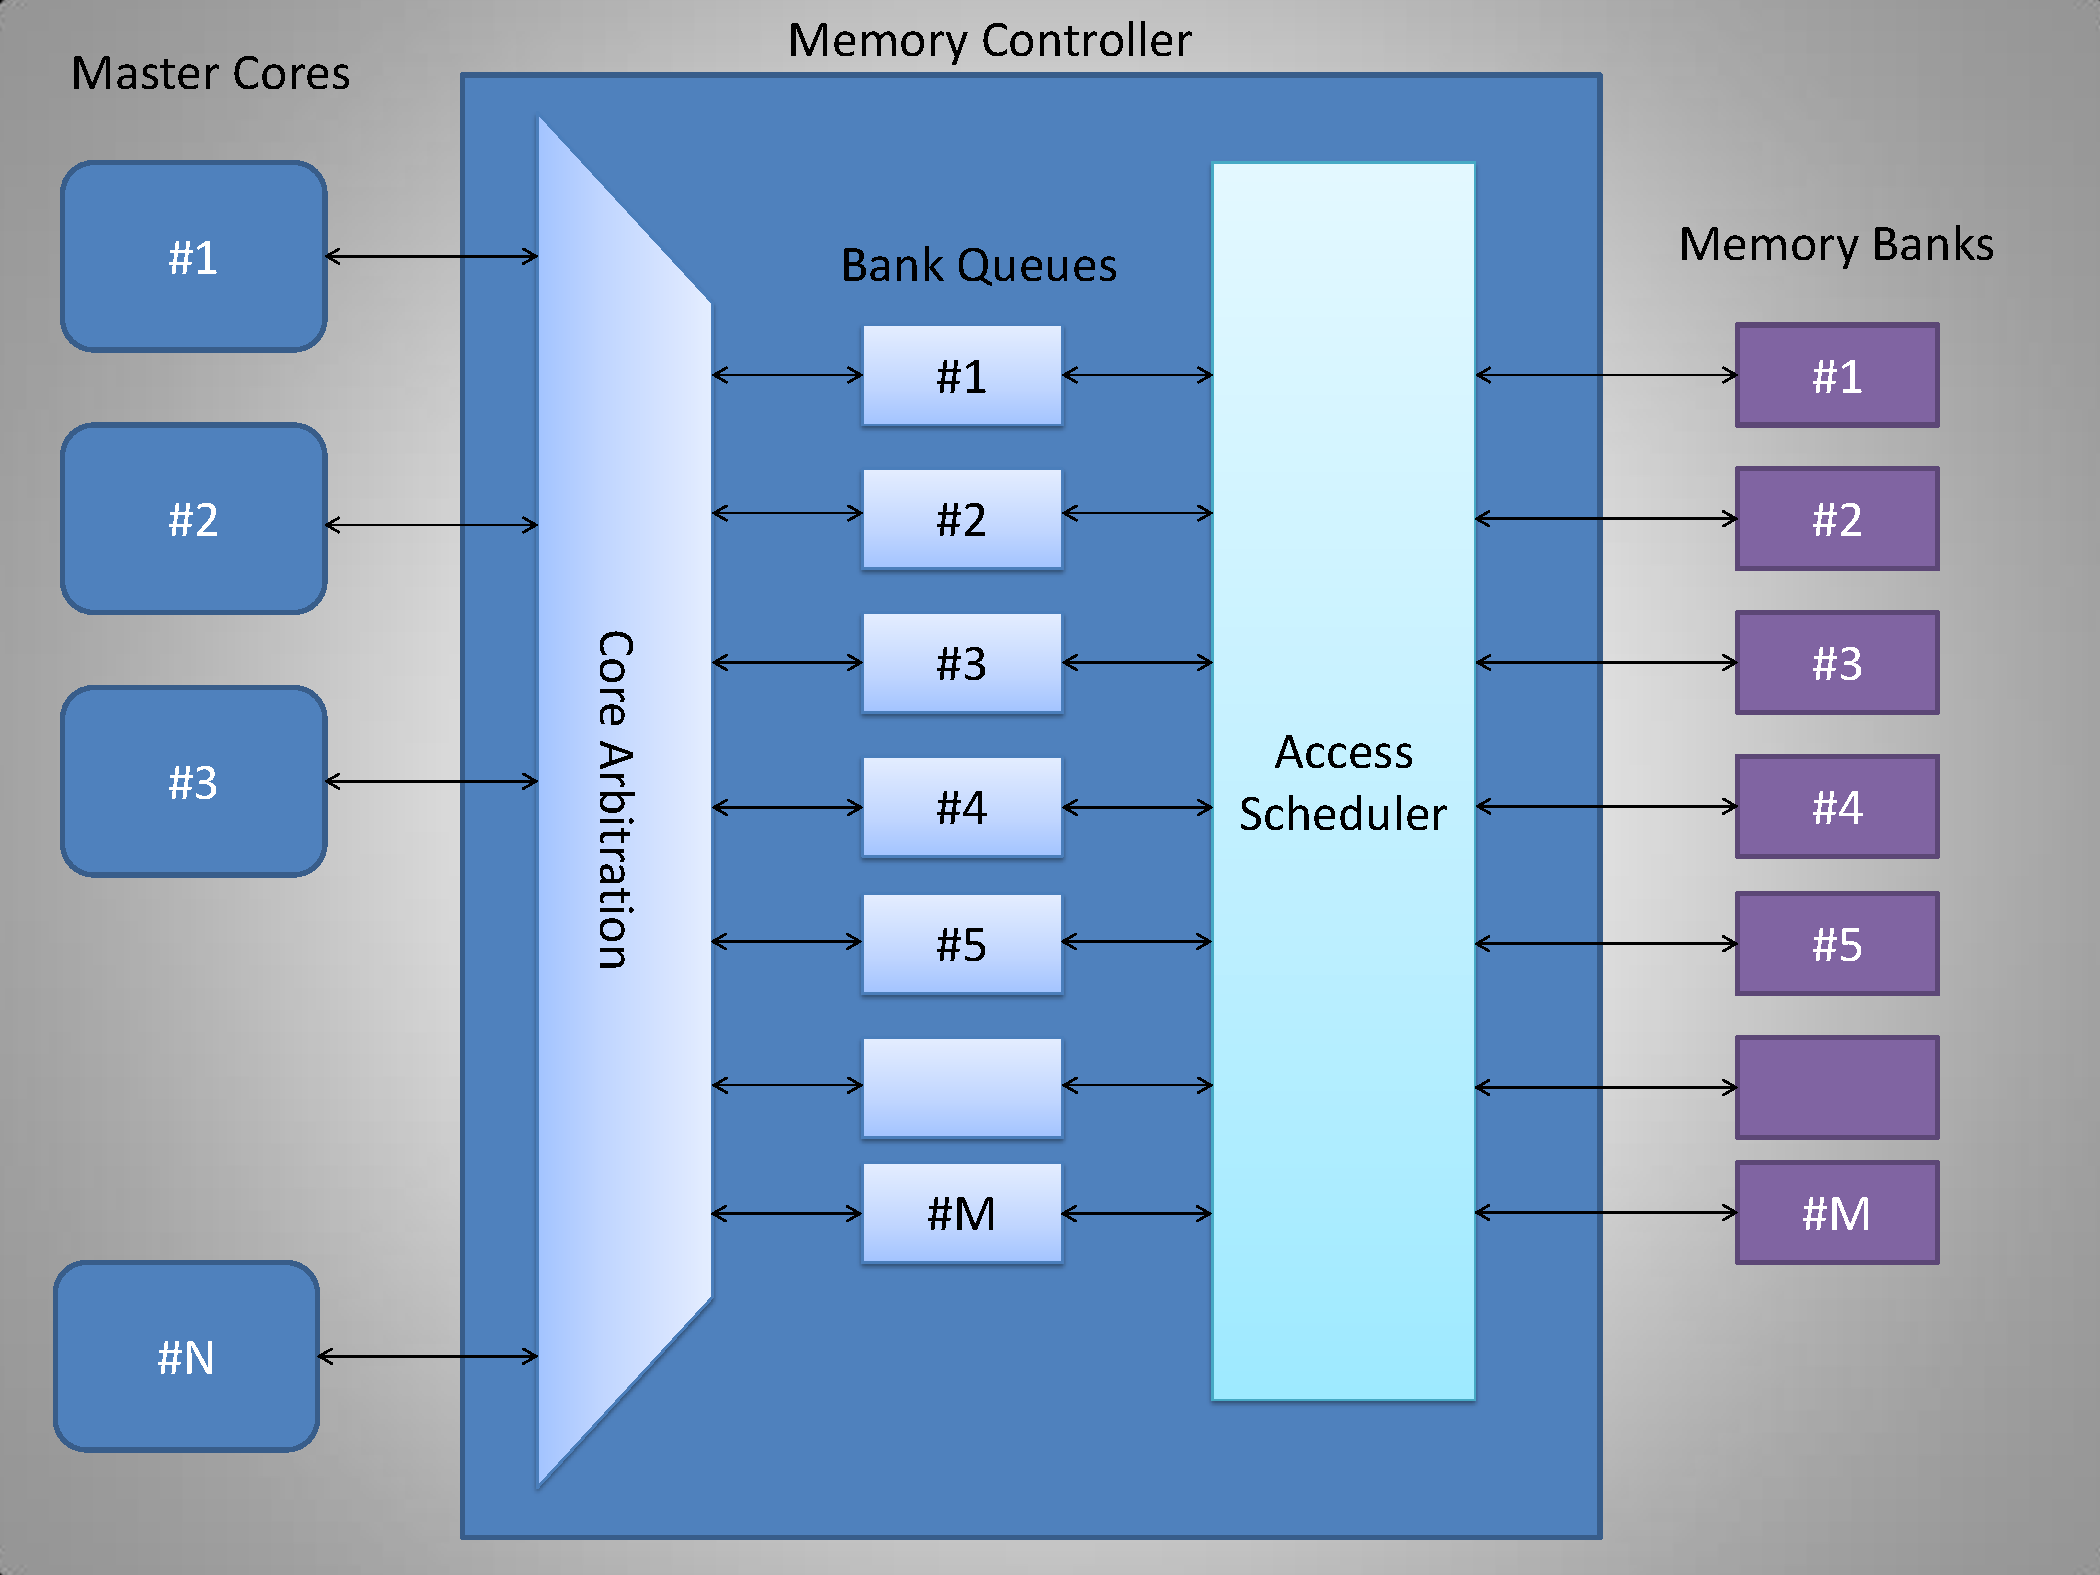
\includegraphics[width=0.7\linewidth]{fig/controllerArchitecture.pdf}
\caption{
{Architecture of Memory Controller} }
\label{fig:pseudo-code}
\end{figure}
%-------------------------
\begin{itemize}
\item \textbf{Core arbiter:~}Every clock cycle, the core arbiter receives up to one request from each core which it stores in an internal queue. The core arbiter attempts to push these request to the appropriate bank queue. If in attempting to push a request the core arbiter detects that the destination bank queue is full, the controller signals that the core is busy which stalls the core. The core arbiter is also responsible for arbitration among the access requests. It arranges the requests stored in its internal queue using a two-step priority order mechanism. It arranges the request in order of QoS priority, and it arranges requests with the same QoS priority using round-robin scheduling.
\item \textbf{Bank queues:~}Each data bank has a corresponding read queue and write queue.  The core arbiter sends memory requests to the bank queues until the queues are full. In our simulations, we use a bank queue depth of 10. 

In addition to the read and write banks, there is a single queue in the bank queues structure which hold special requests such as memory refresh requests.
\item \textbf{Access scheduler:~}The access scheduler is responsible for scheduling access to the various memory banks in the storage space. Every memory cycle, the access scheduler chooses to serve read requests or write requests and algorithmically determines which requests in the bank queues it will schedule. The algorithms the access scheduler uses to choose which requests to schedule are called pattern builders. Every memory cycle, the access scheduler invokes either the read pattern builder or the write pattern builder to schedule read or write requests respectively. A key design trade-off of the pattern builder algorithms is the relationship between the complexity of the access scheduler and the efficiency of the memory access scheduling.

We note that the first two components of the memory controller, i.e., core arbiter and bank queues, in the setting with coded memory banks should not differ much from those in the traditional setup with uncoded storage space. The access scheduler directly interacts with the memory banks and must be designed with our proposed coding schemes in mind. The rest of this section is devoted to discussing the access scheduler in detail.
\end{itemize}

{\color{red} We note that the first two components of the memory controller, i.e., core arbiter and bank queues, in the setting with coded memory banks should not differ much from those in the traditional setup with uncoded storage space. It's the third component, access scheduler, that directly interacts with the array of memory banks and it should take the underlying coding scheme into account while scheduling both read and write requests.} In the rest of this section, we discuss various parts of the access scheduler in detail.

%-----------------------
\begin{figure}[tbp]
\centering
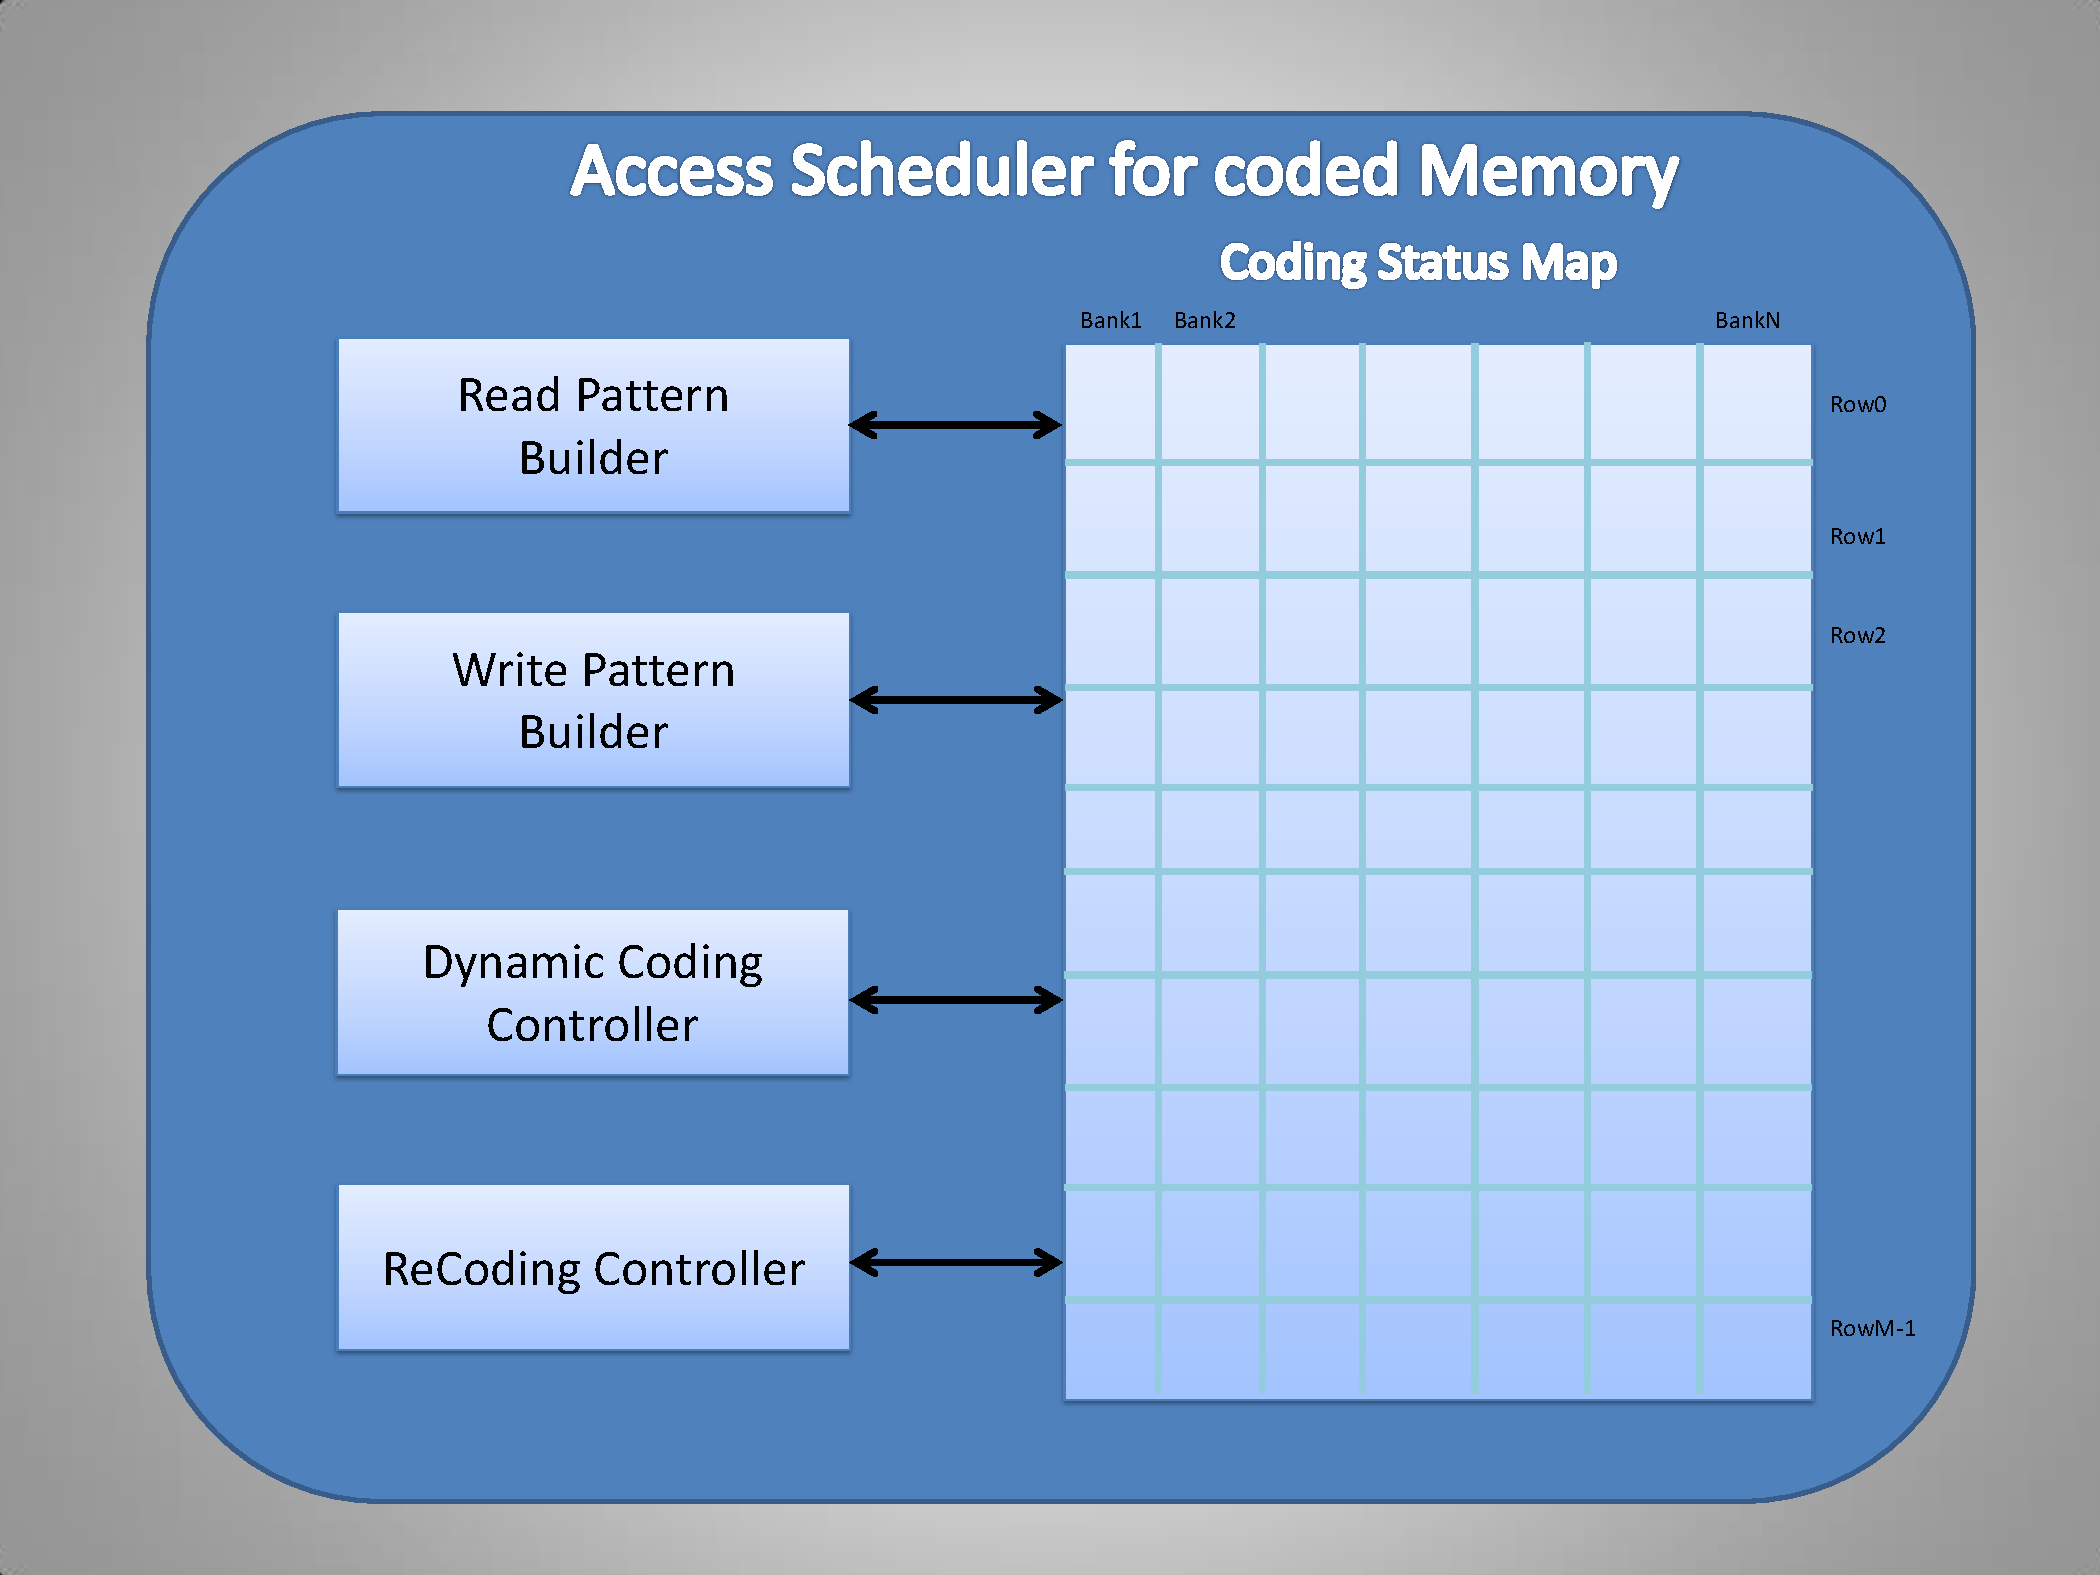
\includegraphics[width=0.7\linewidth]{fig/coded_access_scheduler.pdf}
\caption{
{Access scheduler for coded memory} }
\label{fig:coded_access_scheduler}
\end{figure}
%-------------------------
\subsection{Code Status Table}
\label{sec:codeStatusTable}
The code status table keeps track of the validity of data stored the data and parity banks. The access scheduler may serve a write request using either a data or parity bank. When a write is served to a row in a data bank, any parity bank which uses that data bank to construct coded elements now contains invalid data in the row written to. Additionally, when a parity bank is written to, both the data bank the write request would normally write to, and any parity banks which utilize that data bank contain invalid data in the row written to. The code status table keeps track of where invalid data exists so the access schedule does not erroneously serve read request with stale data, and so the access scheduler can update banks with valid data. 

Figure~\ref{fig:coded_access_scheduler} depicts one implementation of the code status table, and this implementation is the one we use for simulating our proposed memory system. This implementation of thee code status table contains an entry for each row of each data bank. Each entry can take one of three values, either the data in both the data bank and parity banks is fresh, the data bank contains the most recent data, or one of the parity banks contains the most recent data. We assume that the elements of the code status table are accessible at a very fast rate. This implementation of the code status table could be made more effective. 

The implementation of the code status table used in our simulation could be improved. The code status table does not keep track of the intermediate steps the access scheduler takes when rebuilding codes after a write is served. Full knowledge of the status of all data and parity banks allows the access scheduler to serve more requests in some scenarios. Take for example the rebuilding process after a write request is written to a data bank. The access scheduler will rebuilt the elements in all parity banks which use the data bank after the write requests. The code status table will indicate that parities are available for use if and only if all the parity contain updated elements. If some but not all parity banks are updated with rebuilt elements then parity banks can be used, however the access scheduler has no way of knowing which subset of the parity banks contain valid data. The  parity banks containing valid data my go unused when they may have been useful for serving read requests. Keeping track of the status of individual parity banks solves this problem. \Matt{is this example necessary? Is the tangent worth the insight?}


%-----------------------
\begin{figure}[t!]
	%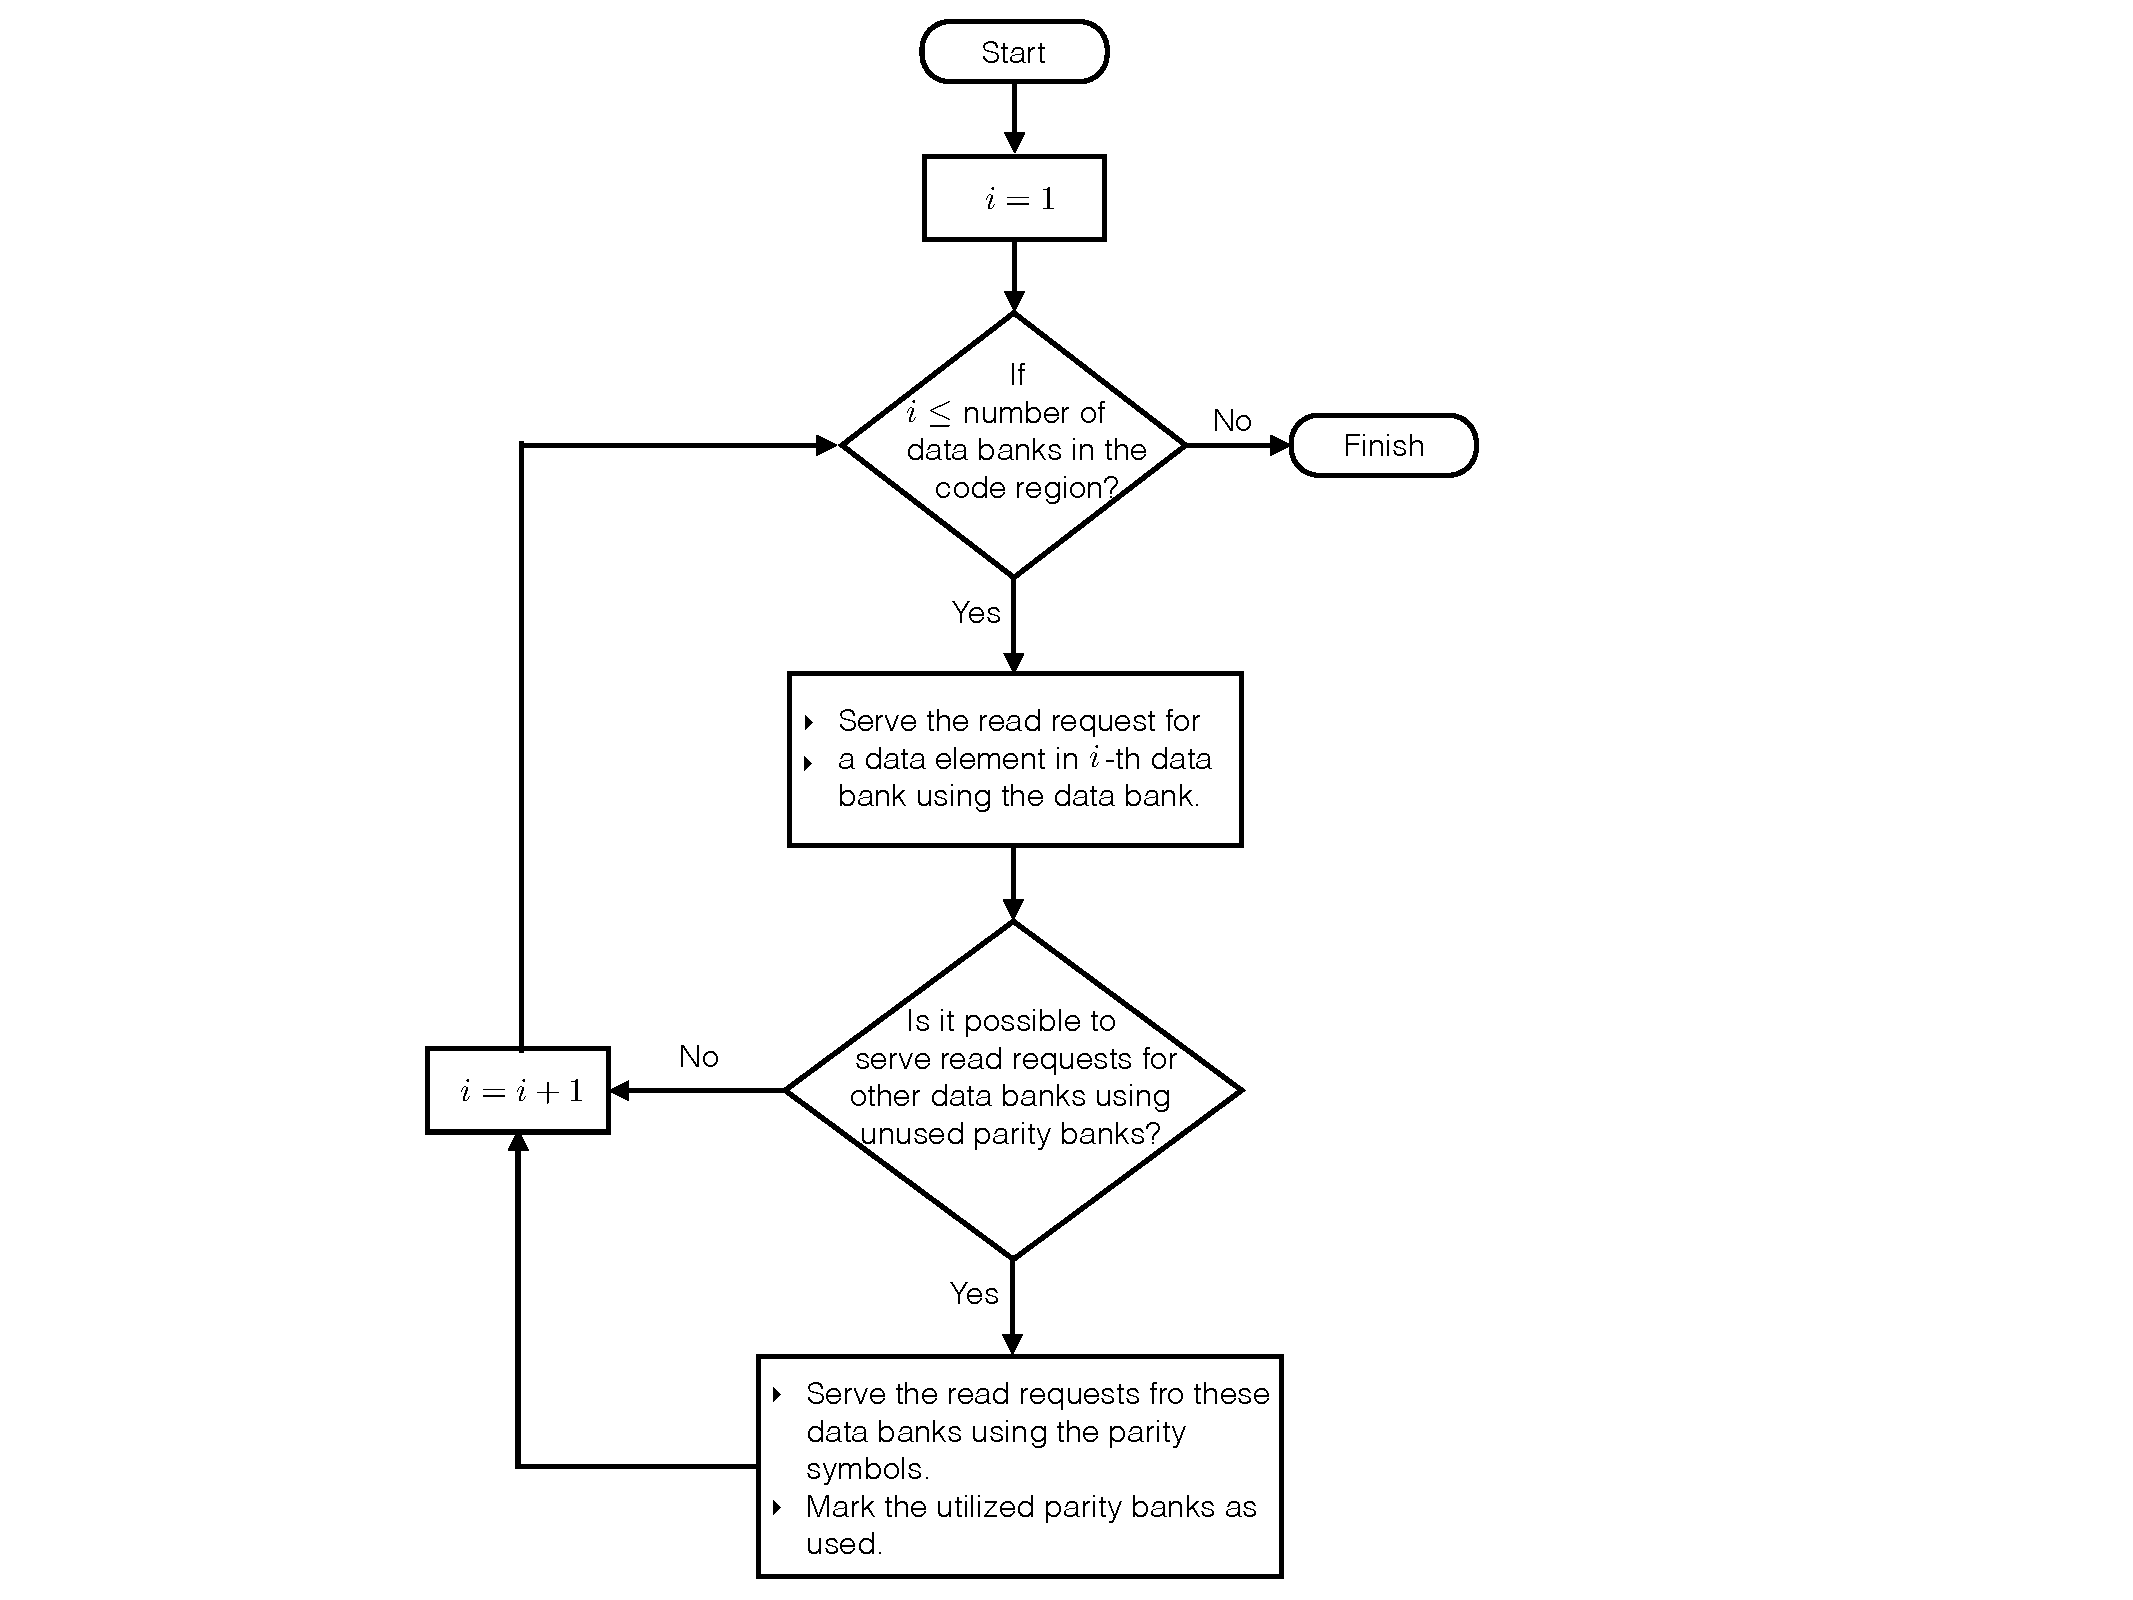
\includegraphics[width=0.9\linewidth]{fig/Read-algo.pdf}
	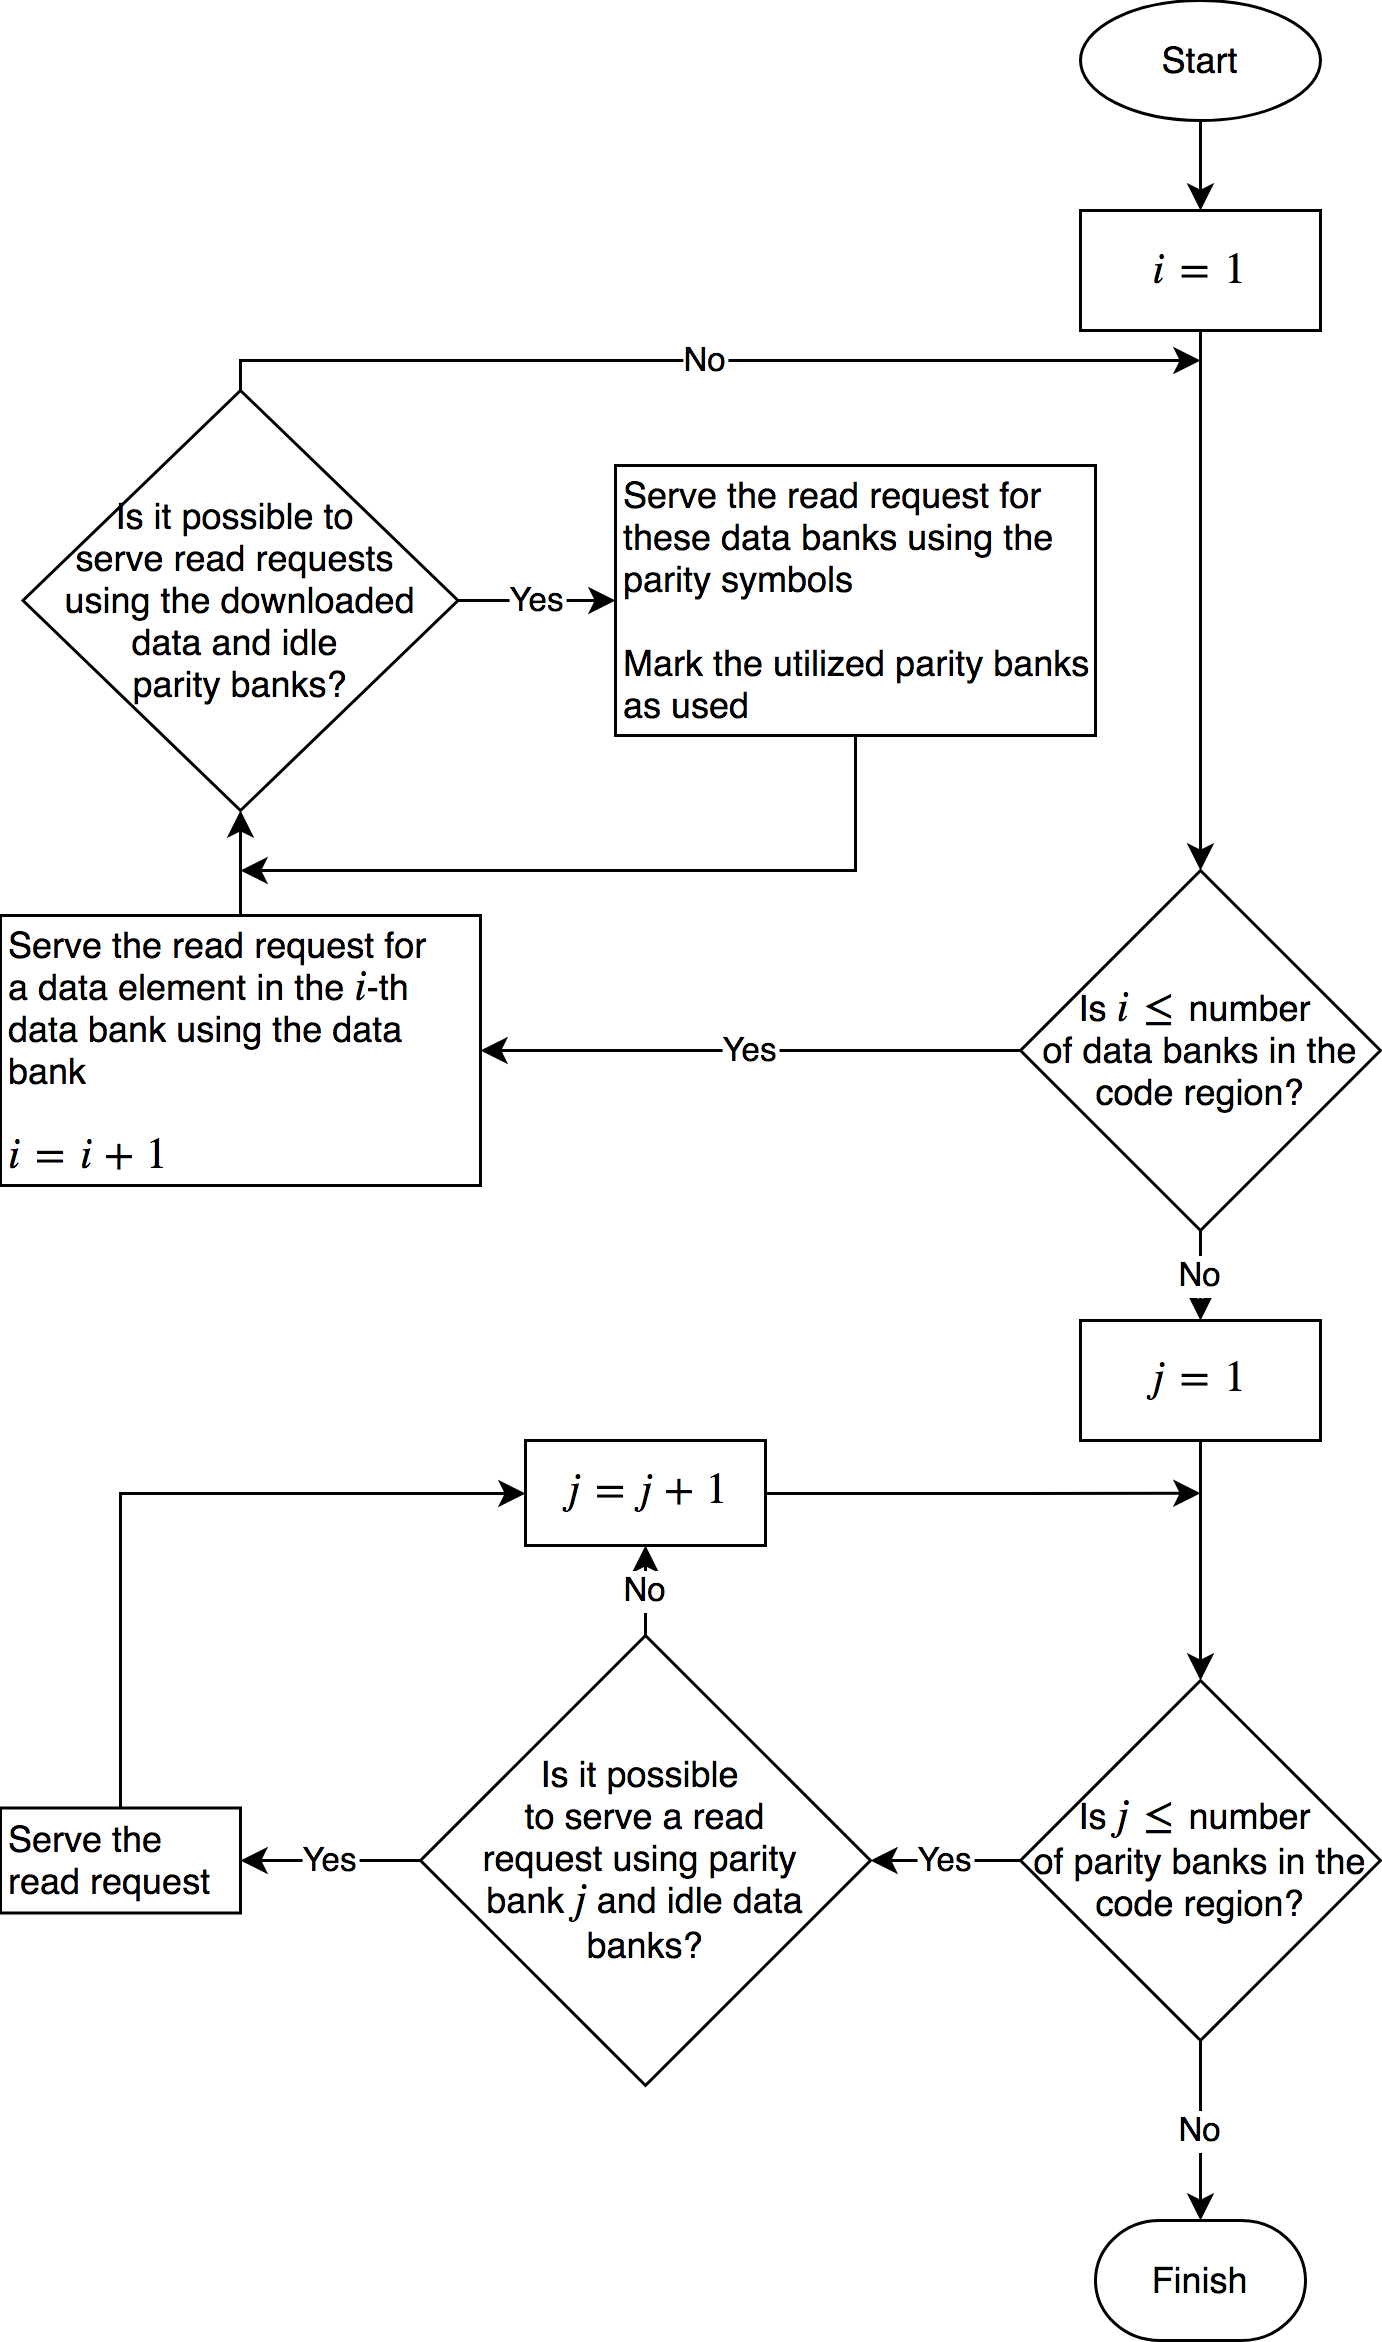
\includegraphics[width=0.96\linewidth]{fig/read_pattern_algo.png}
	\caption{{Description of the algorithm to build a read request pattern to be served in a given memory cycle.}}
	\label{fig:readAlgo}
\end{figure}
%-------------------------
%-----------------------
\begin{figure}[htbp]
	\centering
	%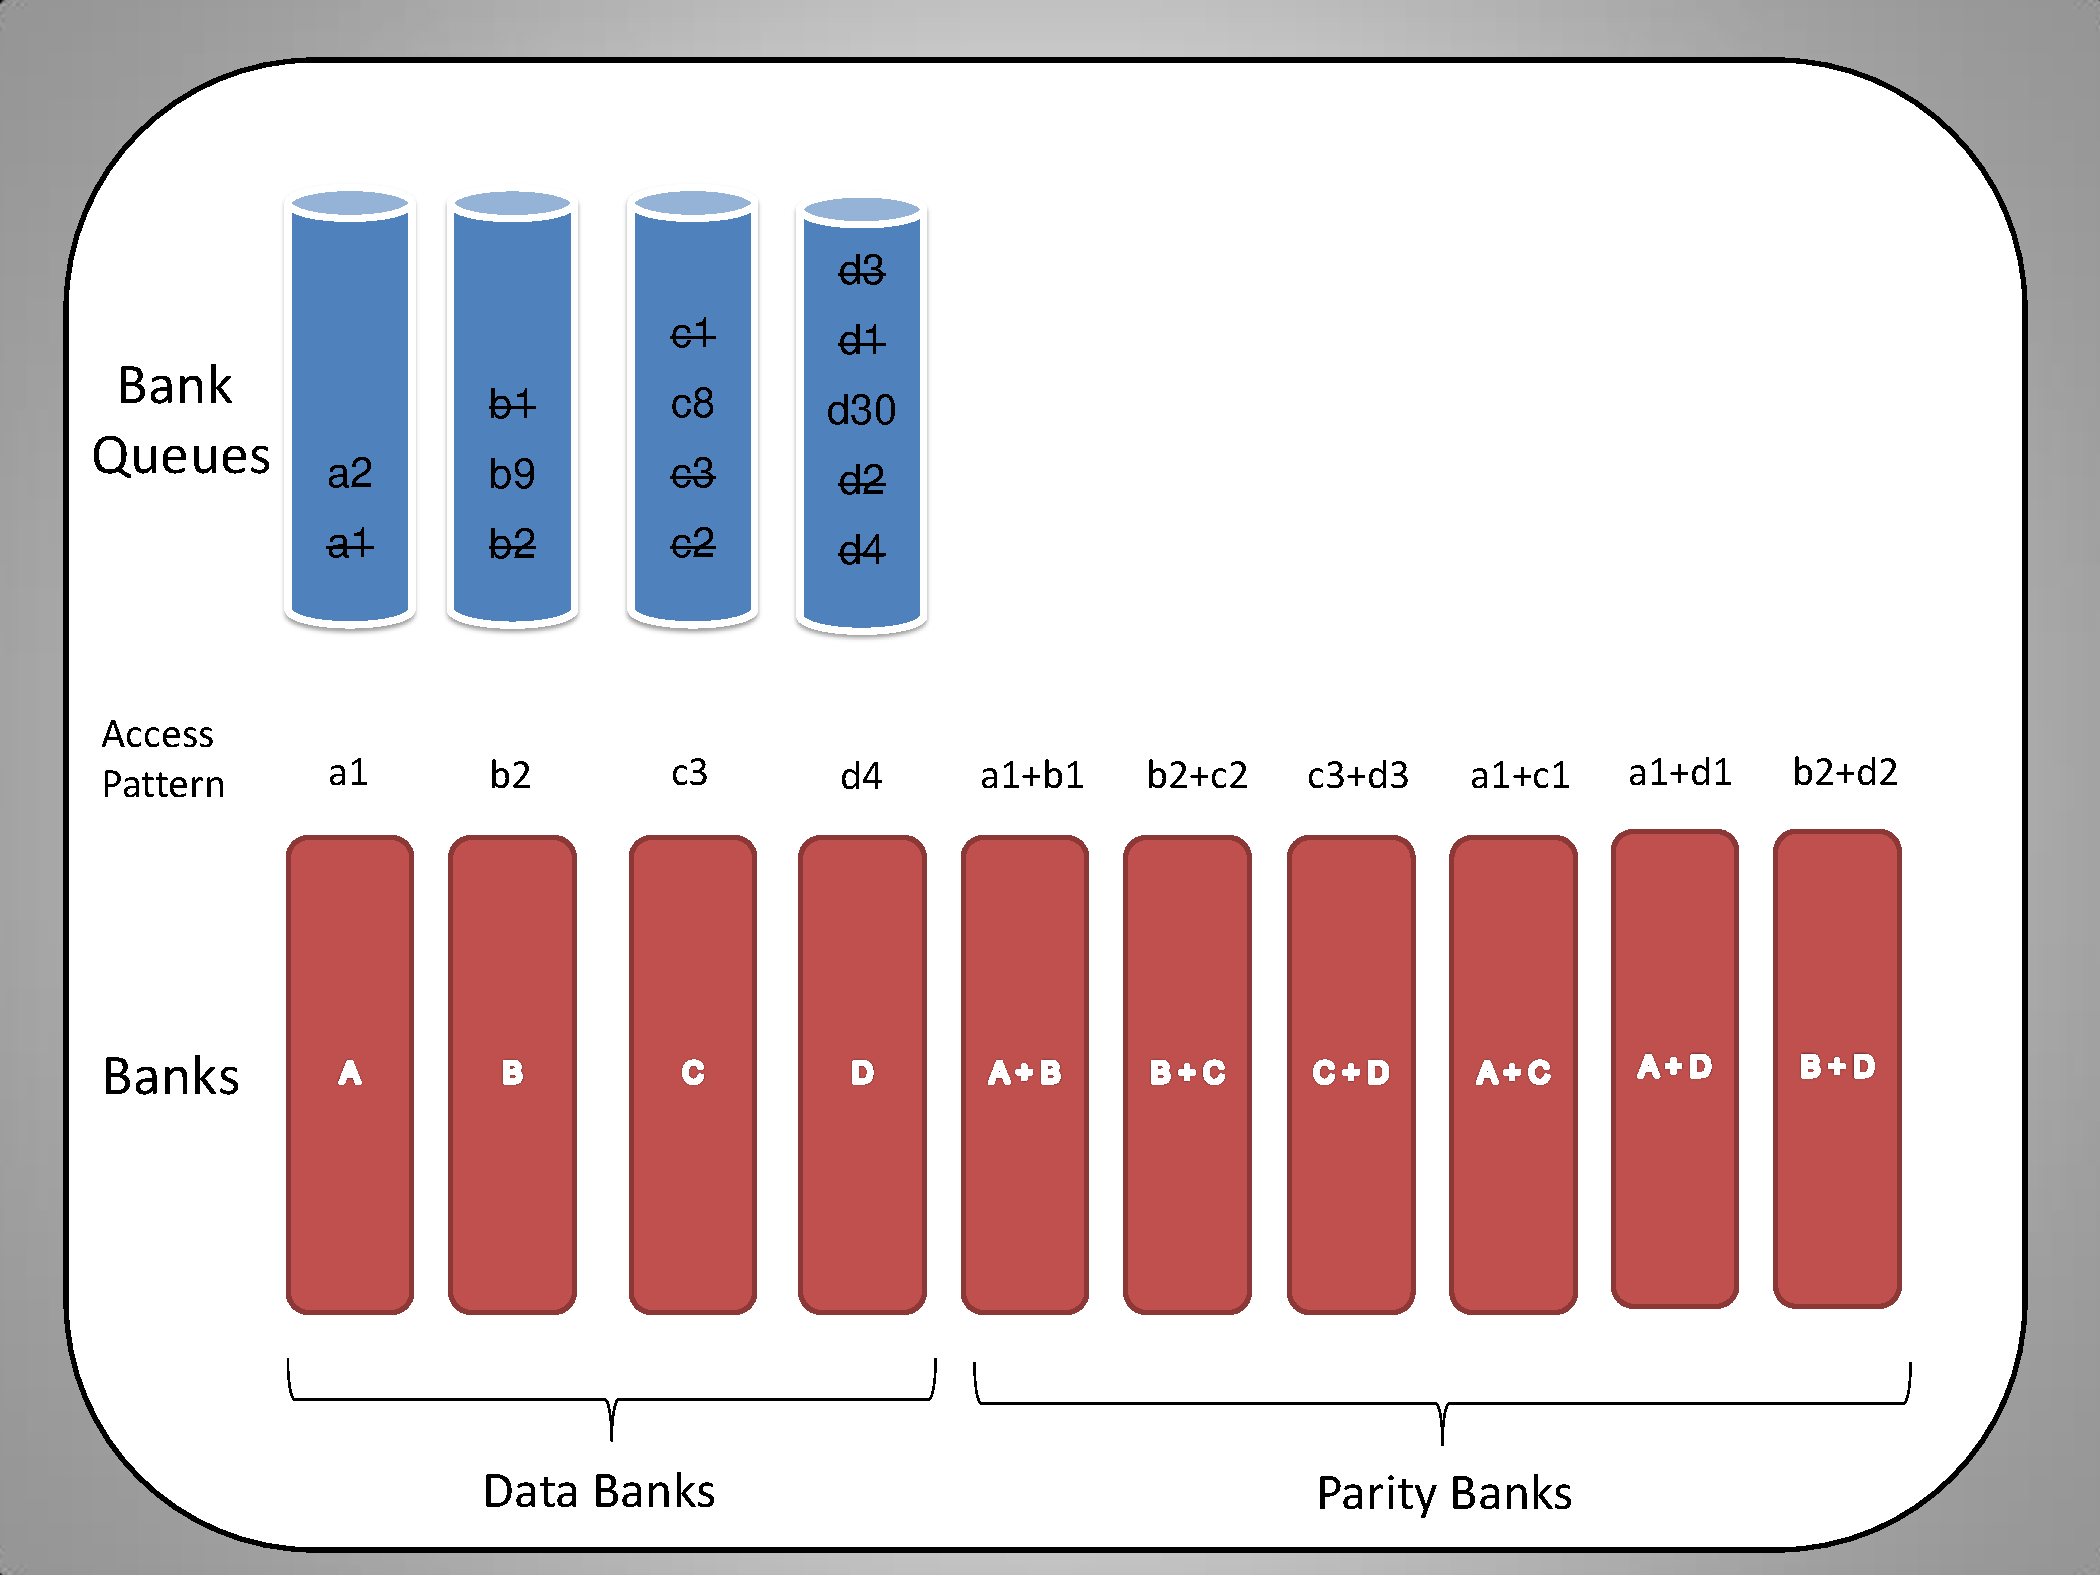
\includegraphics[width=0.7\linewidth]{fig/readAlgoAccessPattern.pdf}
	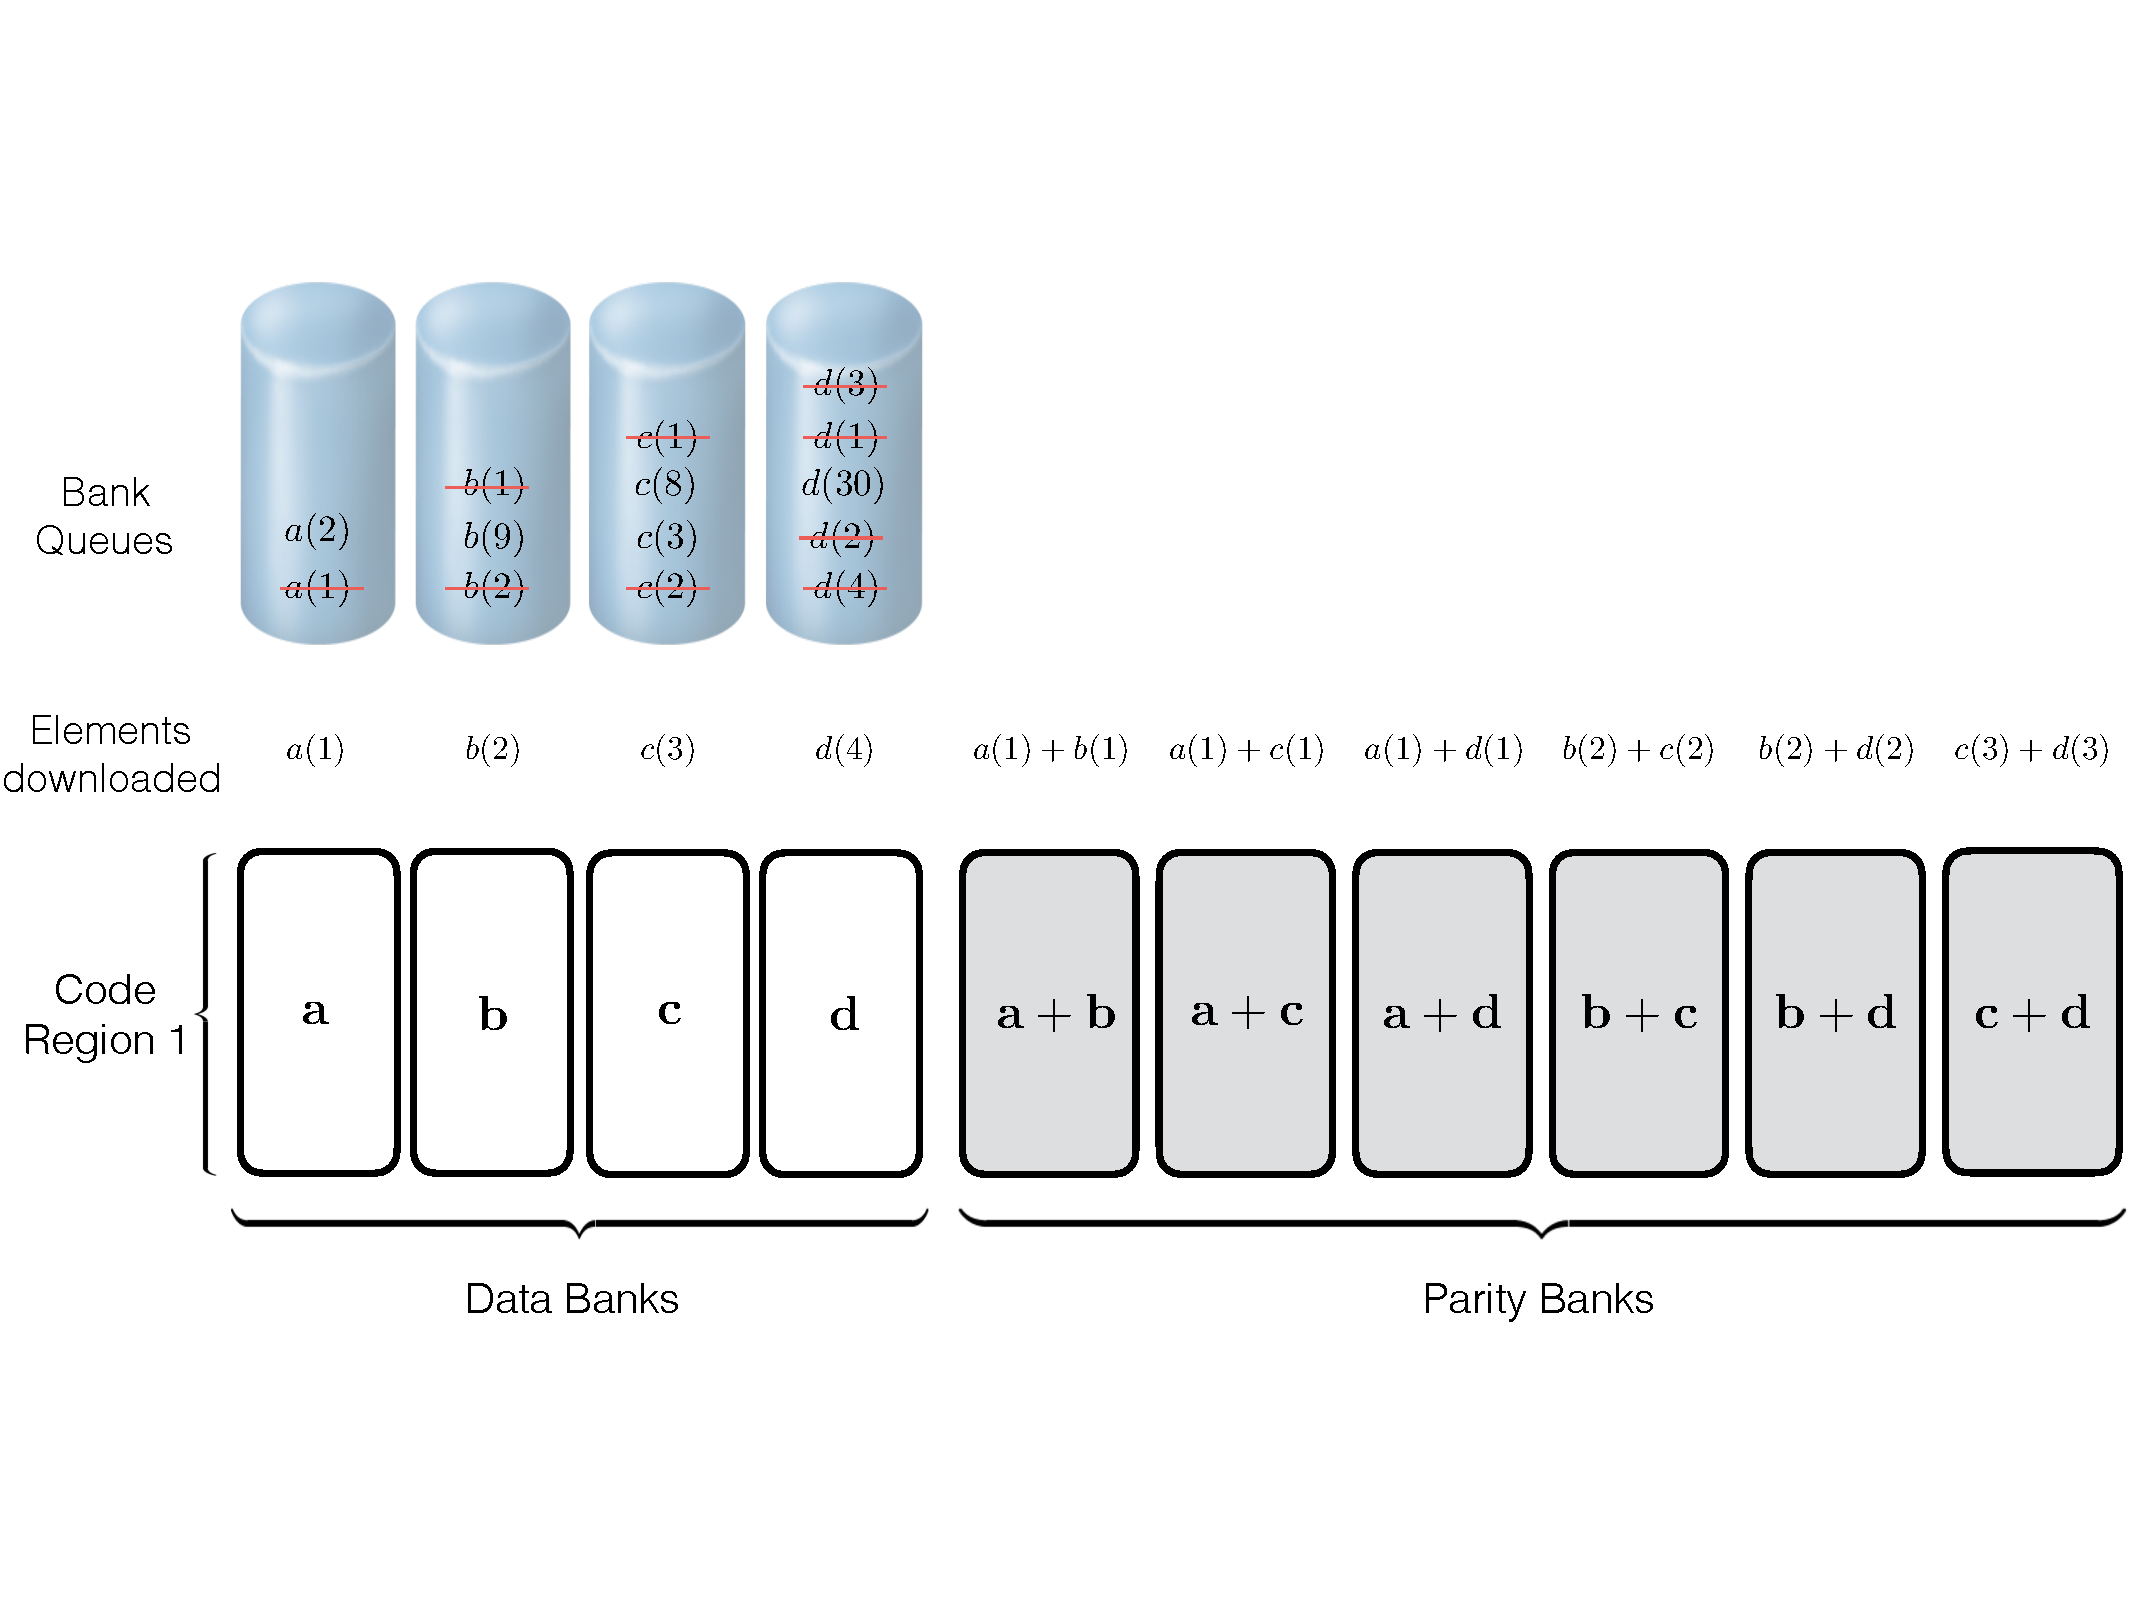
\includegraphics[width=0.96\linewidth]{fig/Read-Algo-Example.pdf}
	\caption{{Illustration of the algorithm to build a read request pattern to be served in a given memory cycle. All the read requests associated with the strikethrough elements are scheduled to be served in a given memory cycle. The figure also shows the elements downloaded from all the memory banks in order to serve these read requests.}}
	\label{fig:readAlgoAccessPattern}
\end{figure}
%------------------------
%\subsection{Read Algorithm for Coded Memory system}
\subsection{Read pattern builder}
\label{sec:readCodingAlgo}
A principal goal of the proposed memory system is to serve many read requests in a single memory cycle. The redundant memory provided by the parity banks gives the memory controller the potential to serve more read requests in a single memory cycle. It is the job of the access scheduler to execute that potential. When serving read requests, the access scheduler selects a set of requests to be scheduled from the bank queues. In order to select the set of requests to be scheduled, the access scheduler must determine how the memory requests will be served by the data and parity banks. Serving a memory request from a data bank is straightforward, because  the symbols in the data banks are at any time ready to be read as long as the code status table indicates that the memory in the data banks is up-to-date. Serving a memory request using a parity bank more complex, because parity banks which contain coded symbols must use symbols downloaded from data banks in order to be decoded. The access scheduler uses the read pattern builder algorithm to determine which requests to serve using parity and data banks. \Matt{is the introduction of the paragraph too wordy?}

The read pattern builder selects which memory requests to serve and determines how requests served by parity banks will be decoded. The algorithm is designed to serve many read requests in a single memory cycle. Figure \ref{fig:readAlgo} is one possible implementation of the read pattern builder. It is important to note that the algorithm depicted will not always schedule the maximum number of read requests in a single memory cycle. The implementation of the read pattern builder shown here is the implementation we use in our simulations described in sections 5 and 6. 

Figure ~\ref{fig:readAlgoAccessPattern} shows the algorithm depicted in one scenario. First, the read pattern builder marks $a(1)$ to be read from data bank $\mathbf{a}$. It then looks through banks $\mathbf{b}$, $\mathbf{c}$, and $\mathbf{d}$ searching for requests for requests for rows $b(1)$, $c(1)$, or $d(1)$ because these symbols can be decoded from a parity bank using the $a(1)$ symbol. In this scenario $b(1$), $c(1)$, and $d(1)$ are all present in the bank queues and are served using parity banks. Symbols equal to  $a(1) + b(1)$, $a(1) + c(1)$, and $a(1) + d(1)$ are all downloaded from parity banks and decoded with $a(1)$. Next, $b(2$) is read from a data bank. Similar to before, $c(2)$ and $d(2)$ are served using parity banks. Again as before, $c(3)$ is read from data bank and $d(3)$ is decoded using $c(3)$. Finally, $d(4)$ is read from a parity bank. In this scenario, Only the top loop of the read pattern builder as pictured in Figure~\ref{fig:readAlgo} successfully serves reads, but there are scenarios where the bottom loop is useful. 

\begin{remark}
Here we note that the aforementioned approach of maximizing the number of read request being served per cycle does come with a cost.  It 
increases the chances of having {\em out-of-order execution} of memory access requests. This does not pose a problem in the case when the memory requests go out of order for different cores. However, in order to prevent the out-of-order execution of the access requests arising from the same core, the logic needs to take care of in-order execution of requests from each cores. We assume that the code arbiter only admits requests into the bank queues if the requests do not pose a threat of out-of-order execution.

\end{remark}
\ignore{
%-----------------------
\begin{figure}[htbp]
\centering
	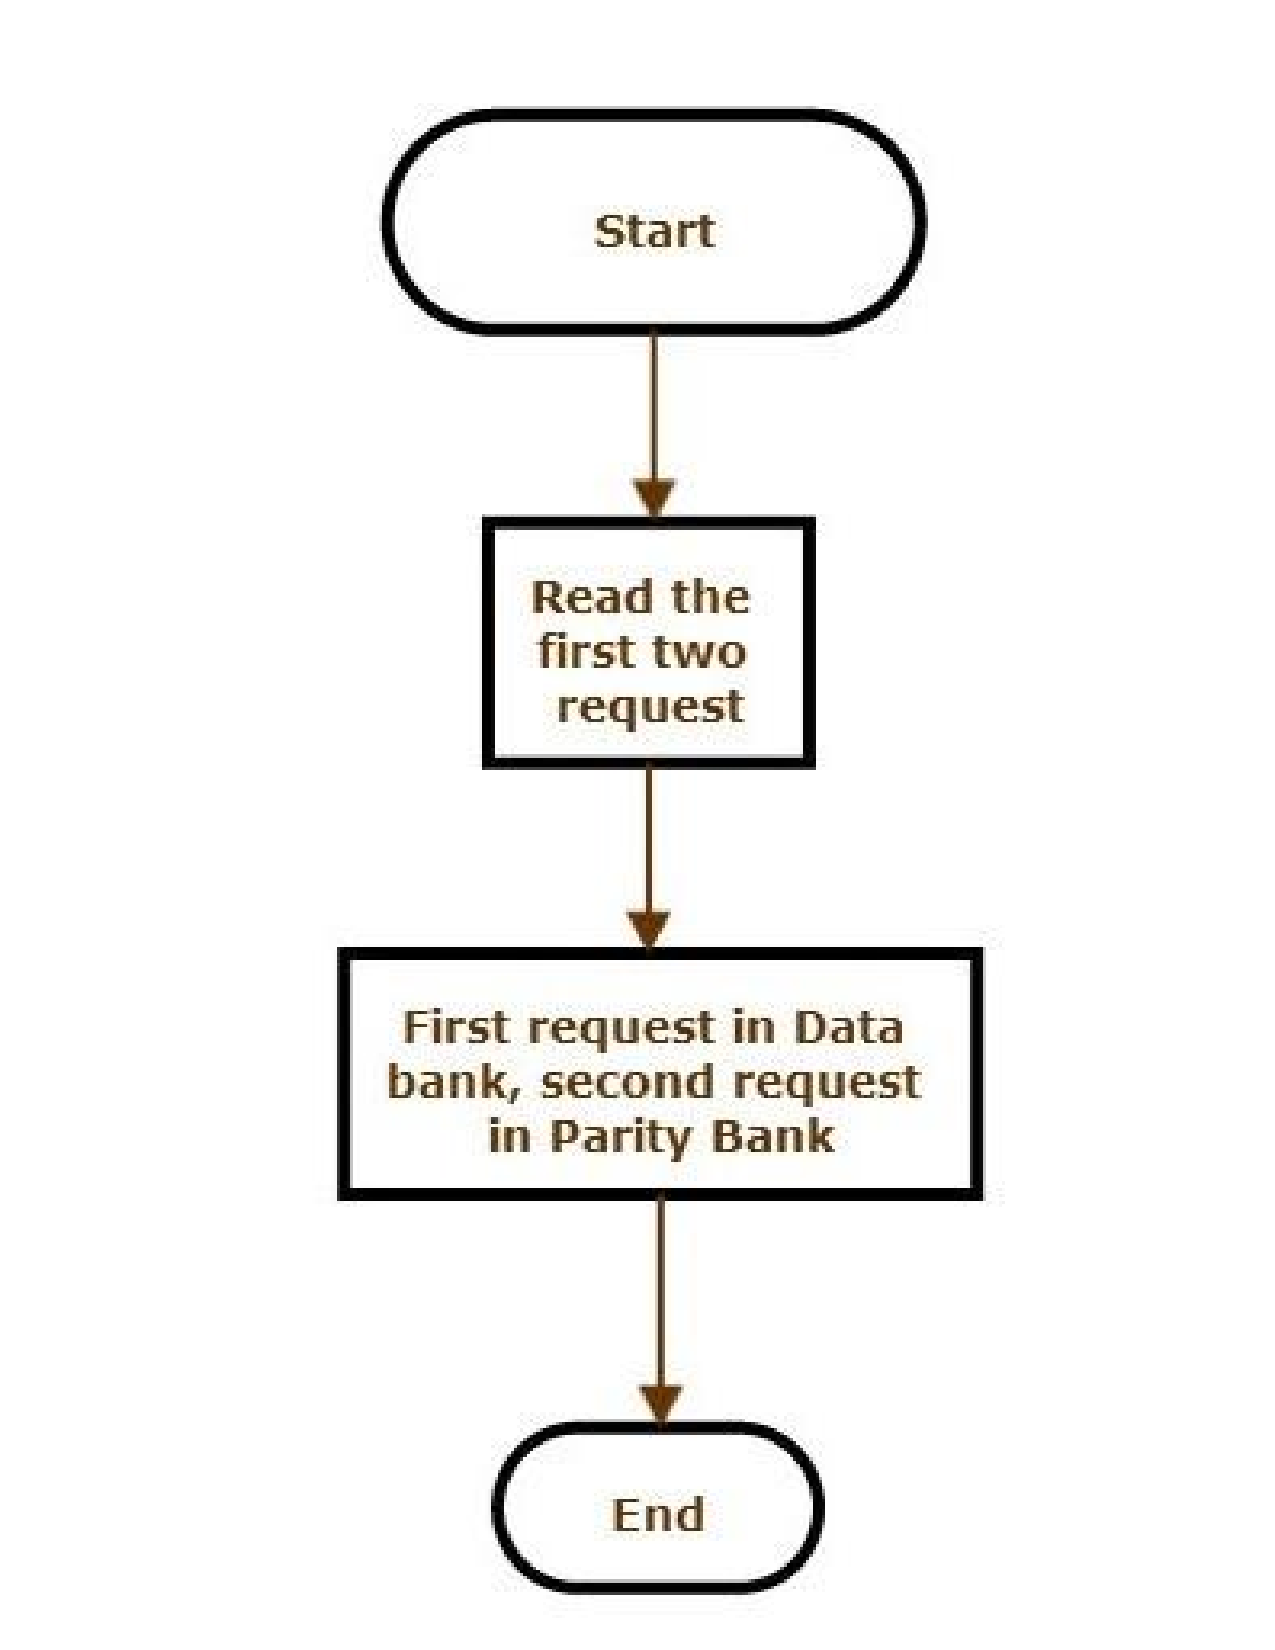
\includegraphics[width=\linewidth]{fig/writealgo.pdf}
	\caption{{\bf Flowchart of Write Algorithm}}
	\label{fig:writeAlgo}
\end{figure}
%-------------------------
%\ignore{
\begin{itemize}
\item Write about how we solve the out of order look ahead problem. If we solve 
	it at all ????
\end{itemize}
}
%\subsection{Write Algorithm for Coded Memory system}
\subsection{Write pattern builder}
\label{sec:writeCodingAlgo}
In addition to the increase in possible read requests per memory cycle, the parity banks allows the memory controller to serve more write requests per cycle. The memory controller serve multiple writes for a single data bank in a single memory cycle by committing some of the writes to parity banks. Similar to the read pattern builder, the access scheduler implements a write pattern builder algorithm which determines which write requests to schedule in a single memory cycle. 

%-----------------------
\begin{figure}[htbp]
\centering
	\includegraphics[width=\linewidth]{fig/write_pattern_algo.png}
	\caption{{ Flowchart of write pattern builder}}
	\label{fig:writeFlow}
\end{figure}
%-------------------------

Figure~\ref{fig:writeFlow} shows a flowchart describing a potential implementation of the write pattern builder. We use this implementation of the write pattern builder in the simulations described in sections 5 and 6. In this implementation, the access scheduler serves write request with lower priority that read requests. Only when the write bank queues are nearly full does the access scheduler run the write pattern builder algorithm. Figure~\ref{fig:writeAlgoAccessPattern} shows how the write pattern builder described in Figure~\ref{fig:writeFlow} works one scenario. Without the parity banks, only one write per data bank is possible, resulting in the service of four write requests. The introduction of parity banks allow for a total of 10 write requests. Note that an element which is destined for row $n$ in a data bank can only be written to the corresponding row $n$ in the parity banks. 

We illustrate the aforementioned functioning of the write pattern builder with the help of an example shown in Figure~\ref{fig:writeAlgoAccessPattern}. In this example, the write queue is full for all the four banks. The controller picks up $2$ write requests from each of these queues and schedules them to be written to the respective data bank and one parity bank. The controller also updates the code status table map with the appropriate status. It updates the writes committed to data bank with $01$ and writes committed to parity bank with $10$. The write build pattern will only serve a write using parity banks if the request's row exists in the parity bank. 

Figure~\ref{fig:writeAlgoAccessPattern} also demonstrates how the code status table changes to reflect the freshness of the elements in the data and parity banks. Here, the 00 status indicates that all elements are updated. The 01 status indicates that the data banks contain fresh elements and the elements in the parity banks must be recoded. The 10 status indicates that the parity banks contain fresh elements, and that the data bank must be updated and the elements in the parity banks must be updated.

\ignore{writes are scheduled to address {\em a2} and {\em a9}. The write to {\em 
	a2} goes to {\em a2}, however, the write to {\em a9} goes to the data 
bank {\em a9 + b9}. This helps us do two writes in one cycle.  However, the 
data bank of {\em a9} still contains the stale value. The scheduler updates the 
{\em coding status} of each row after committing a write. }
%-----------------------
\begin{figure}[t!]
\centering
	%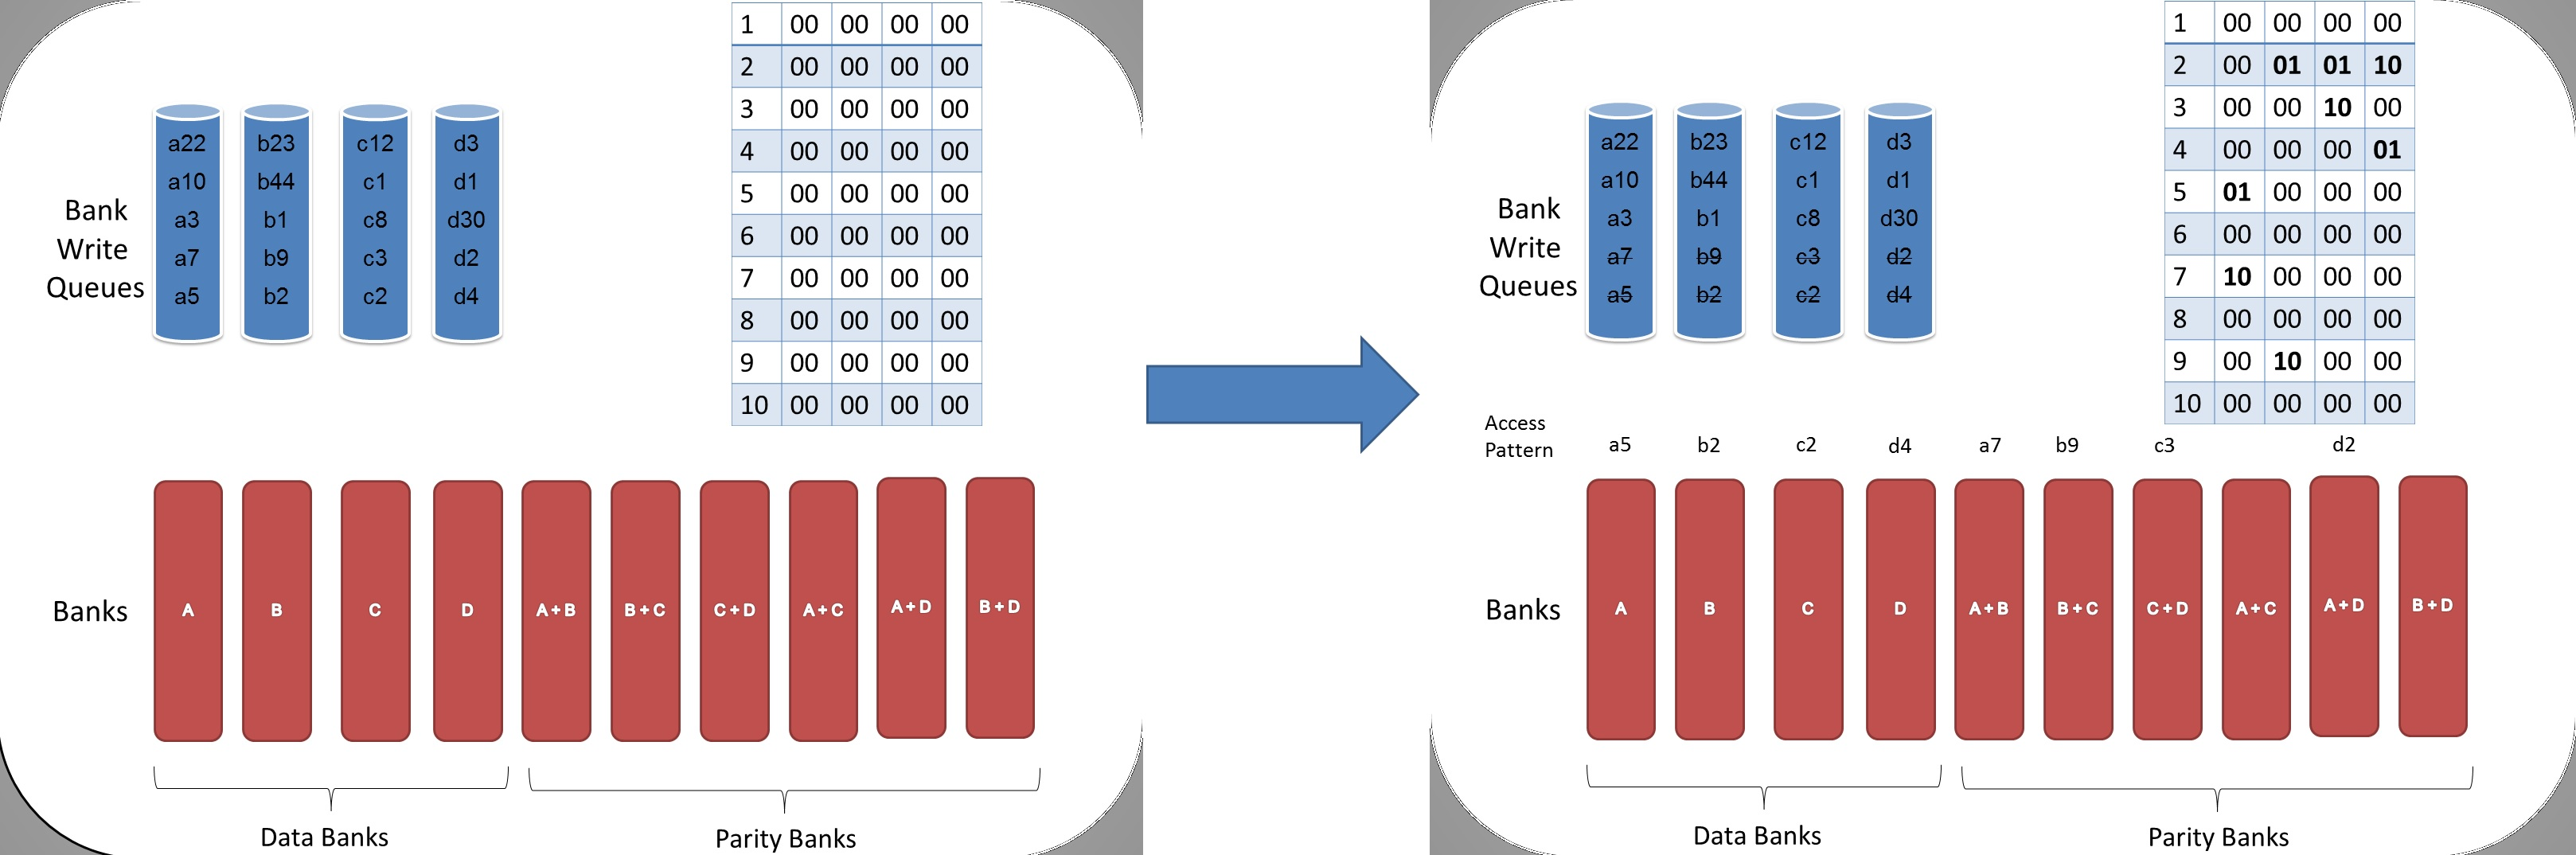
\includegraphics[width=\linewidth]{fig/writeAlgoAccessPattern.jpg}
         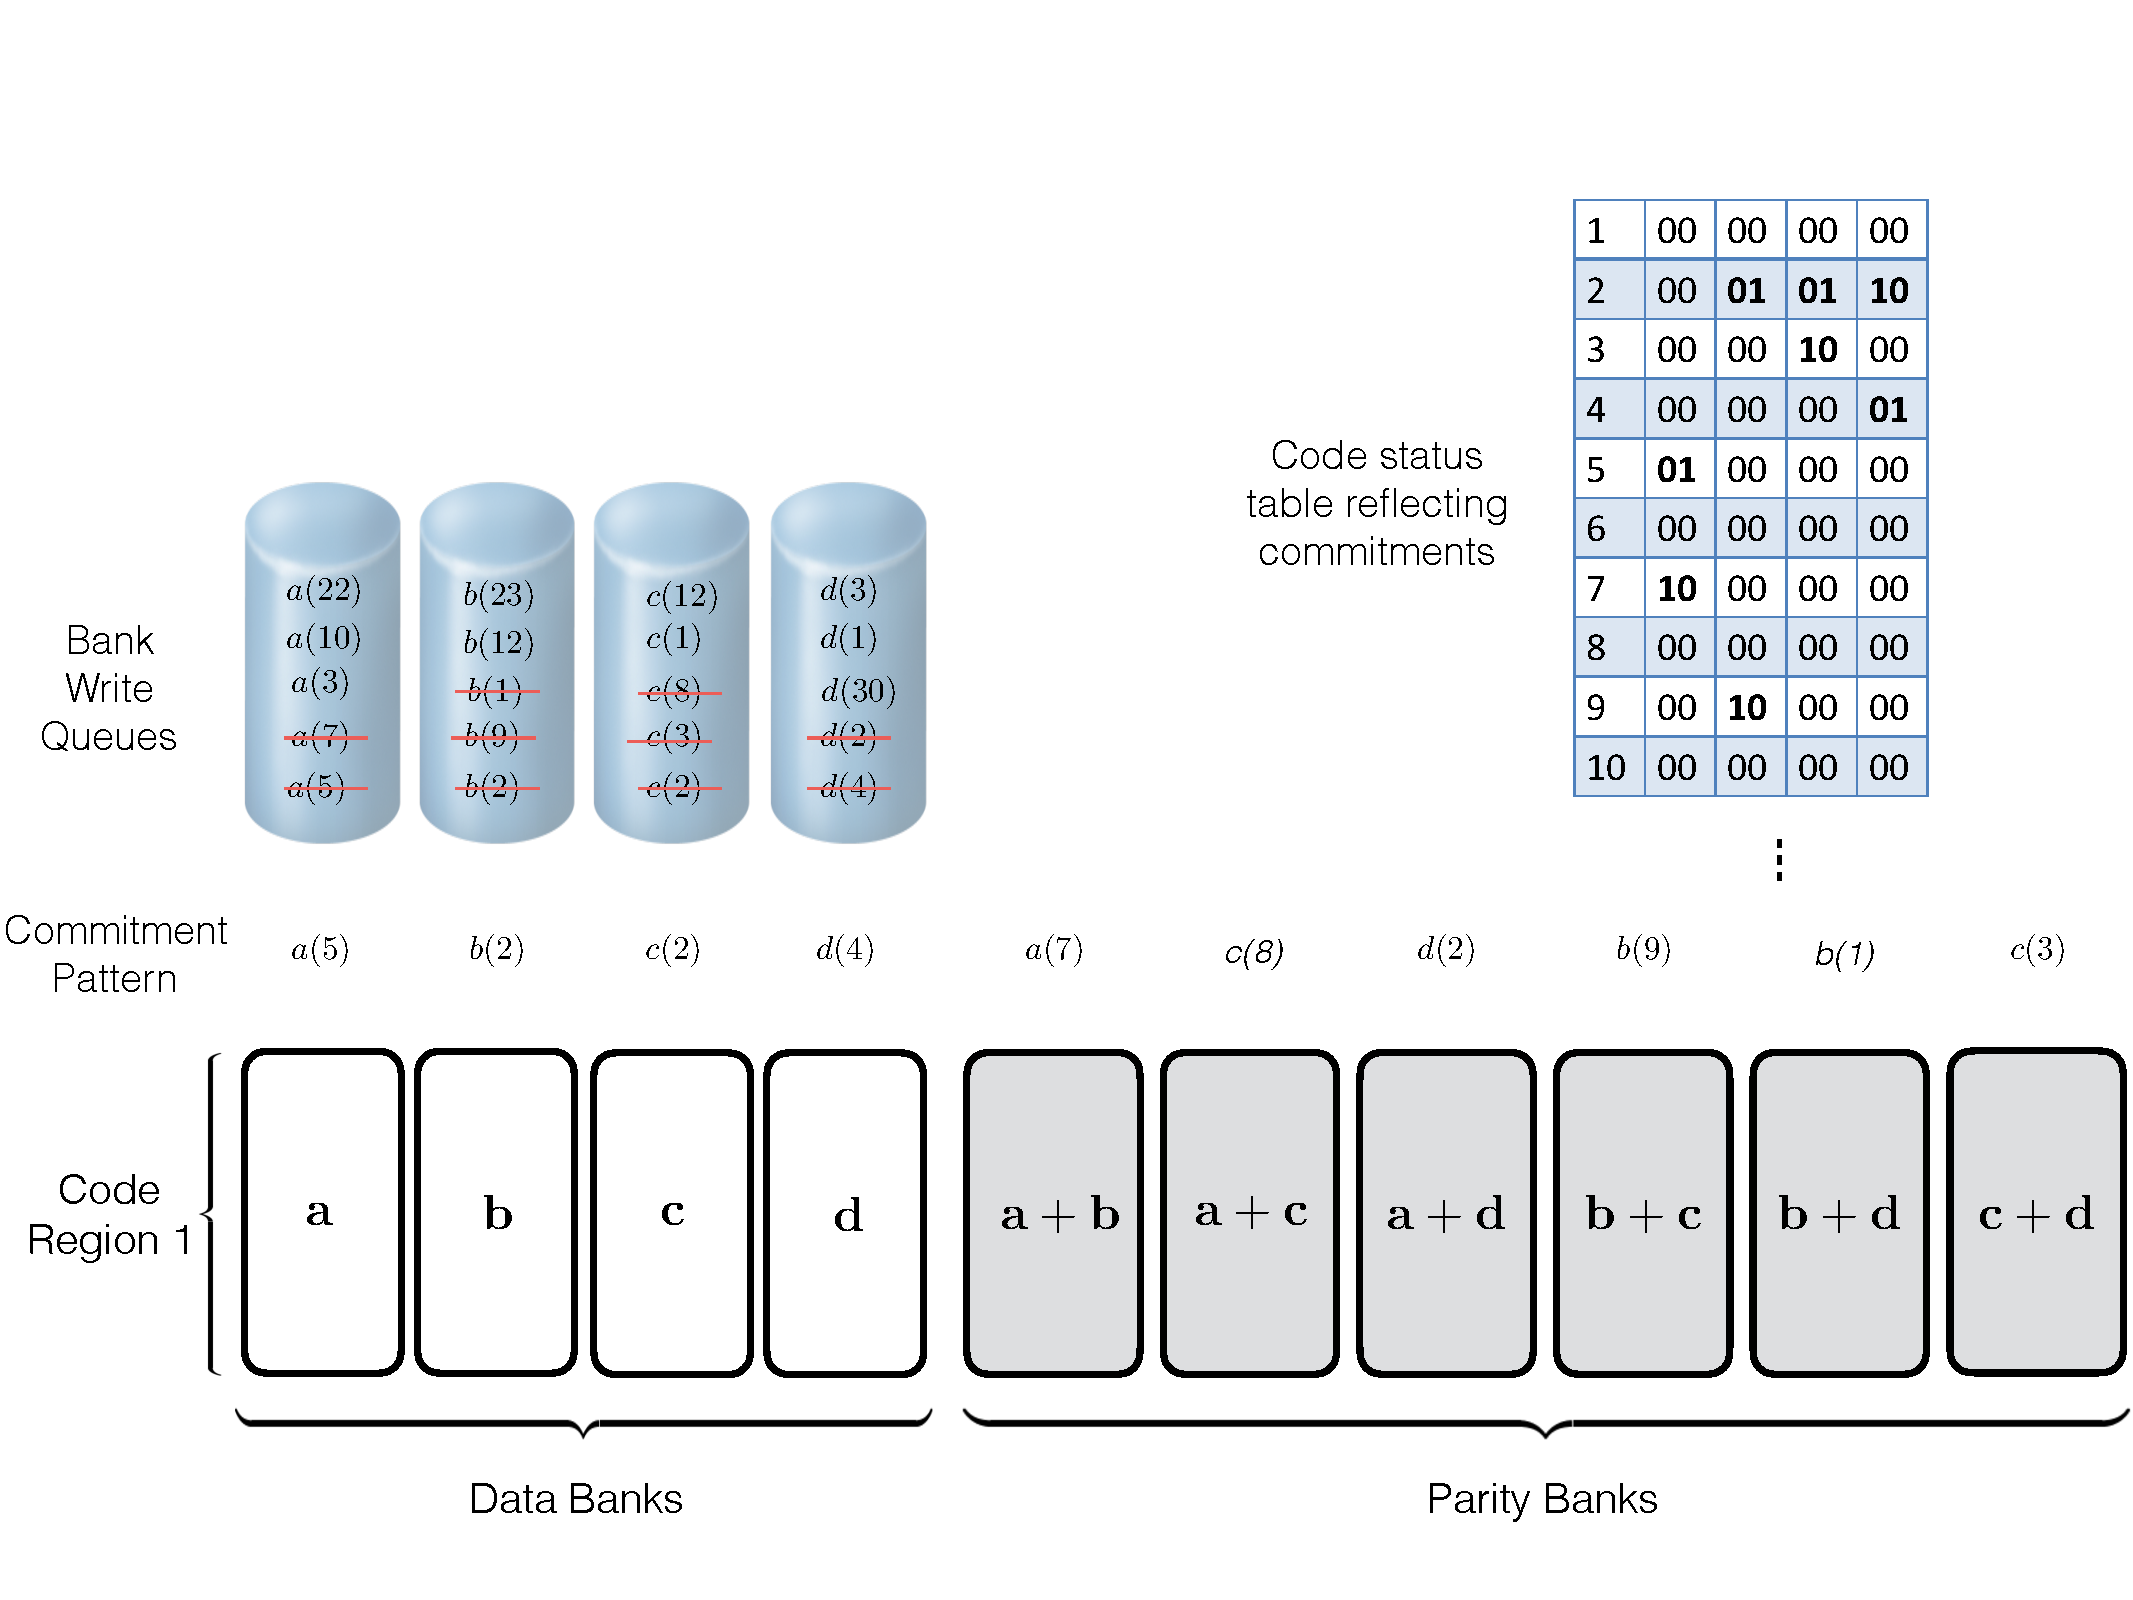
\includegraphics[width=\linewidth]{fig/Write-Algo-Example.pdf}
	\caption{Figure describing write algorithm access pattern}
	\label{fig:writeAlgoAccessPattern}
\end{figure}
%-------------------------
\subsection{ReCoding unit}
\label{sec:recoding}
After a write request has been served, the stale data in the parity or data banks must be replaced. The ReCoding Unit is responsible for updating the elements of data and parity banks after a write is served. The ReCoding Unit contains a queue which is updated every time a write request is served. We calll the elements on the ReCoding Unit queue “recoding requests”. Recoding requests indicate the data and parity banks which contain stale elements, and the bank the write was served to which resulted in the recoding request. The recoding requests also contain the cycle number the request was created so the ReCoding Unit may prioritize older requests. 

The ReCoding Unit downloads the necessary elements needed serve the recoding units from data and parity banks left idle by the read pattern builder and the write pattern builder. In the case of restoring data in a parity bank, the ReCoding unit downloads and stores from the data banks over one or more memory cycles and restores the parity code once all requisite data has been retrieved. For storing a write which has been stored in a parity bank, the ReCoding unit writes the new data to the data bank and then begins to restore the parity code. If during the execution of the read pattern builder or write pattern builder elements are downloaded which are useful for recoding, the element is sent to the ReCoding Unit.


\subsection{Dynamic Coding}
\label{sec:dynamicCoding}
To reduce memory overhead, the size of the parity banks is only a fraction of the size of the data banks. Ideally, the most heavily access portions of memory are the portions which are redundantly stored in the parity banks. The dynamic coding block in the access scheduler is responsible for maintaining codes for the most heavily accessed memory sub regions.

The contention in memory accesses from various cores occurs mostly when the access are to shared-memory, especially when they are localized to certain memory regions. We explore the locality of the memory access over a period of time to reduce the memory overhead for storing the codes. In a multi-core system, when various cores try to work from a shared memory location, they tend to generate accesses to a localized region of memory. This motivates the idea of coding the localized region during the period of heavy access, and dynamically changing the region whenever there is change in the locality of memory accesses. Figure 17 shows the access pattern for an 8-core simulated system running the dedup PARSEC benchmark. The y-axis of the figure shows the address accessed by the cores over a period of time. The x-axis denotes the time in nanoseconds. This plot shows that most of the access from various cores are primarily located in the lower memory band. Greater than 95% of all memory accesses are from this band 18 magnifies this band and reveals that the lower band is composed of two sub-bands of roughly equal density. 


\begin{figure}[htbp]
		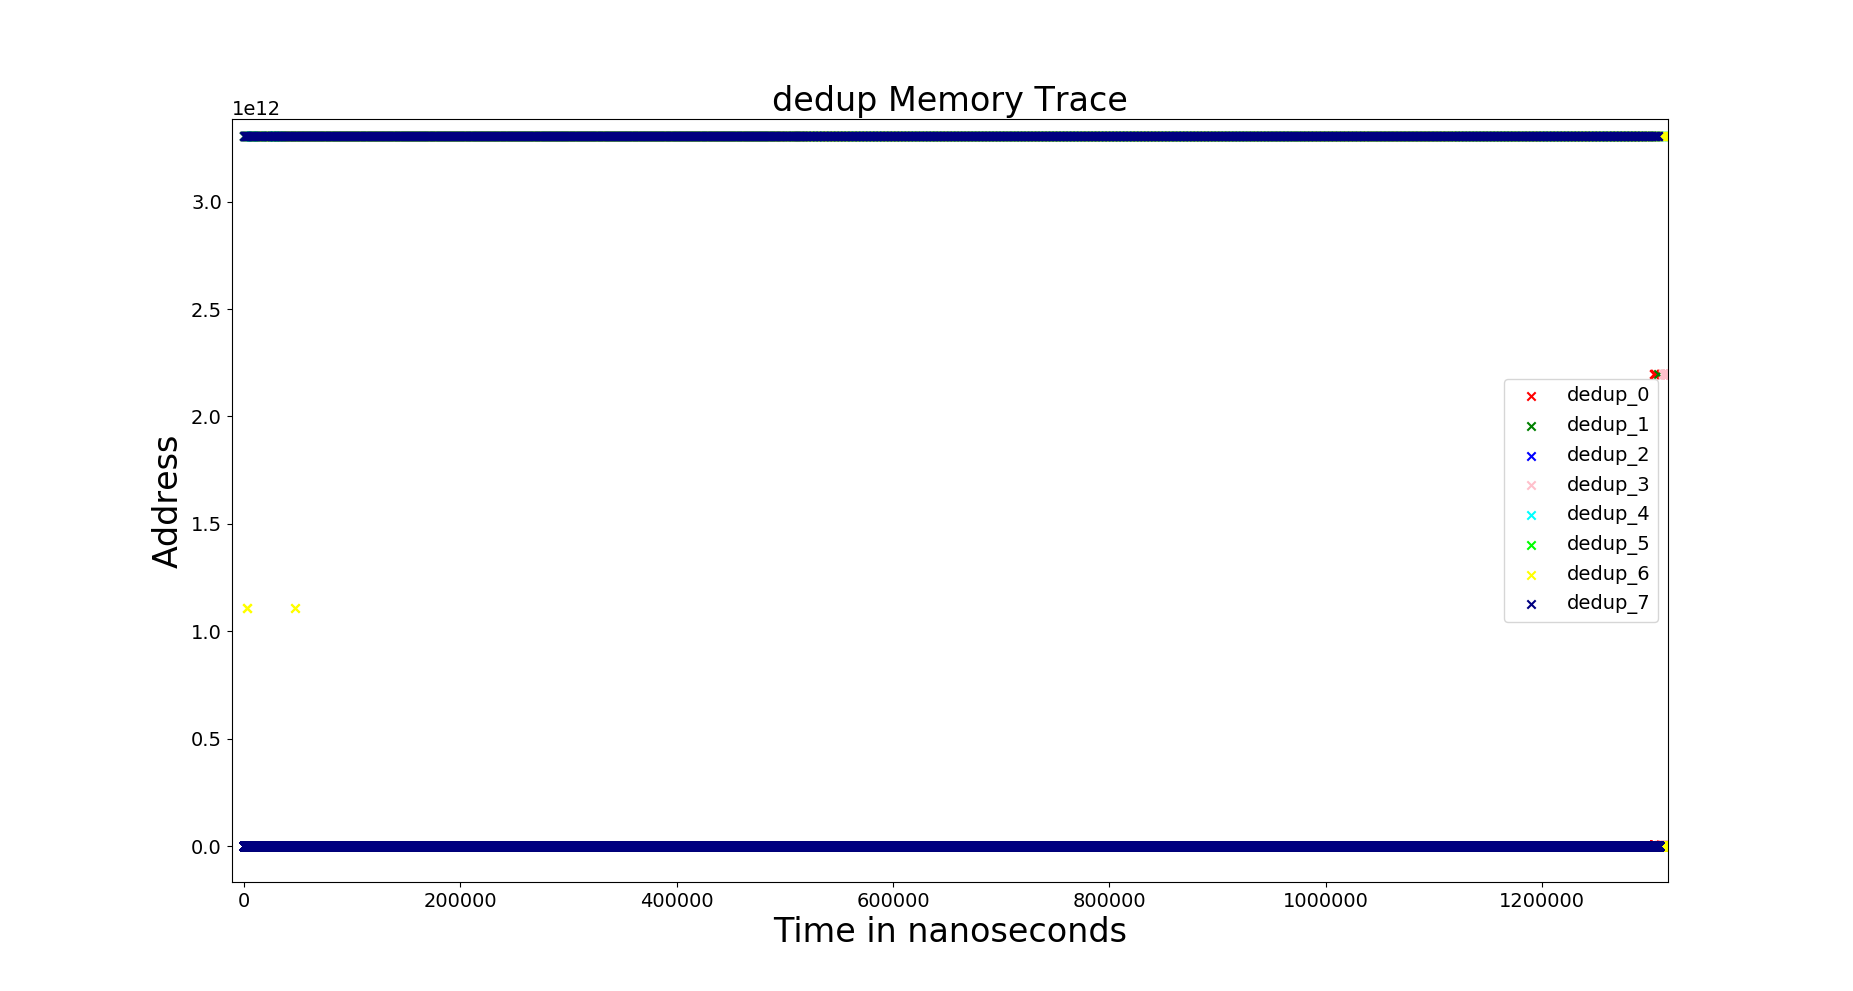
\includegraphics[width=\linewidth]{fig/dedup_whole.png}
		\caption{Memory Access from the Dedup PARSEC benchmark. This trace was generated using 8 cores.}
		\label{fig:dedup_whole}
\end{figure}

\begin{figure}[htbp]
		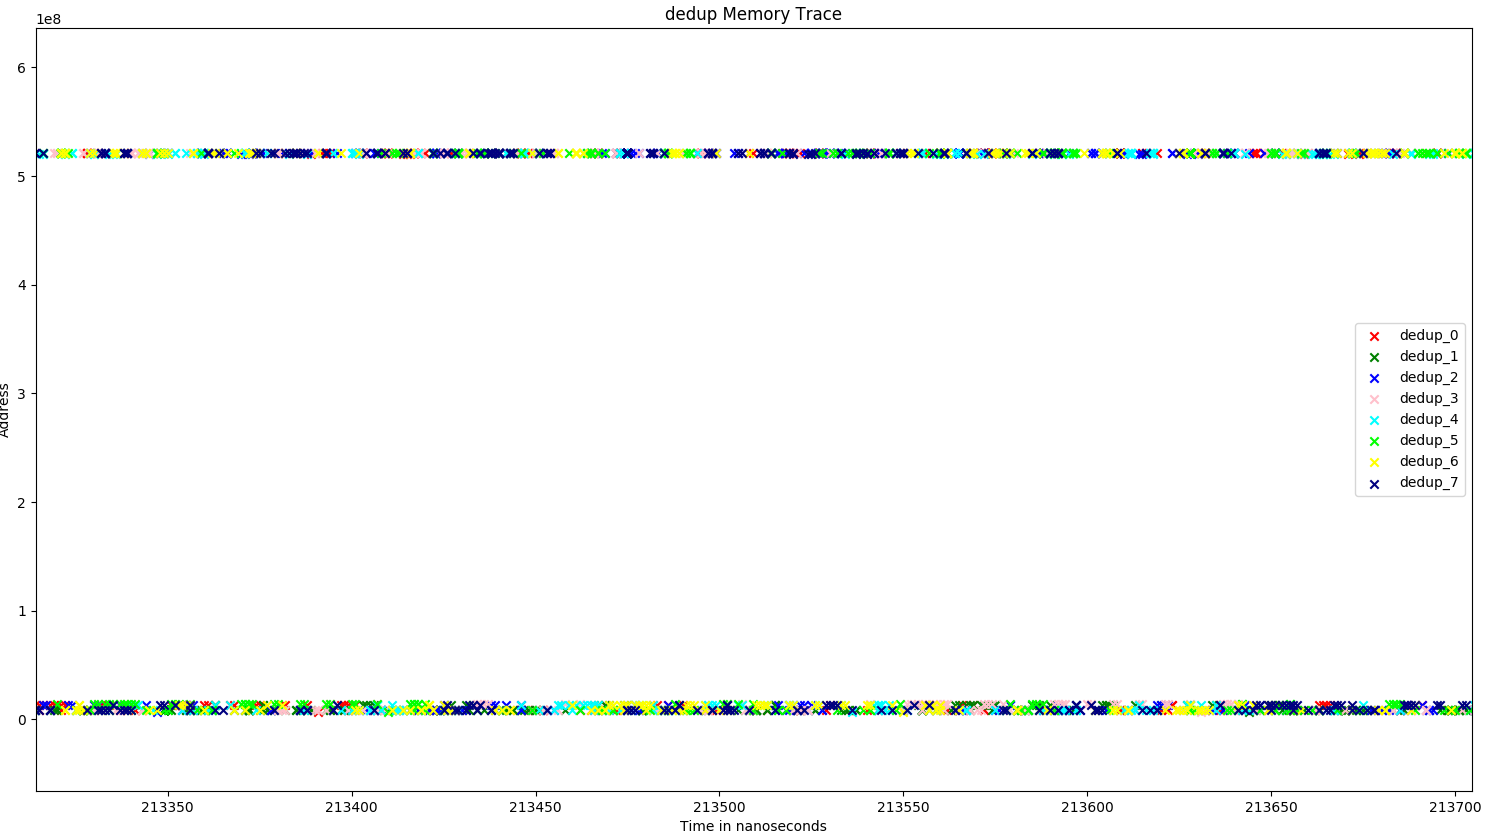
\includegraphics[width=\linewidth]{fig/dedup_dense.png}
		\caption{Memory Access from the Dedup PARSEC benchmark demonstrating the density of memory accesses}
		\label{fig:dedup_dense}
\end{figure}

From these observations, we demonstrate the idea of coding the 
highly accessed portion of the memory. This scheme benefits from a huge 
reduction of the memory overhead with coding. The reduction in the memory 
overhead can be used to reduce the complexity of the decoder by using simple 
coding functions (e.g. xor) and for denser coding (e.g. repeatedly coding a 
single element using 2 elements). 

The scheme of dynamic coding requires that the currently coded region changes 
when the access pattern changes. That is, the localized memory area that is most heavily accessed 
can change, and it will require the system to recode the new localized access 
region. We assume that the working area of a program changes with change in the 
input parameters to the program. It can be easily observed from the above 
figures that the working area or the localized area is constant for at least 1 
ms. This suggests that the switching of the coded region is not very frequent. 
%{\bf During these periods of coding switches, it is also guaranteed that the number 
%of accesses served from the memory is at worst equal to the number of banks 
%available. In other words, coding the memory has no performance degradation 
%compared to non-coding during these times.} The system also needs to maintain an 
%algorithm to observe the access pattern of the cores, and make a decision when 
%it is time to code a new memory region. To do this, the memory controller tracks 
%the most accessible region during a time period and makes a decision to 
%slide/shift the coded region. This shift in the coded region requires the update 
%of the parity bank for the new region. This process is carried out in 
%conjunction with the ongoing access to the newly coded region. Therefore, this 
%operation only requires writes to the parity banks, since we can use the current 
%reads from the coded region to access the data that is to be coded. In addition, 
%reads are also scheduled in the idle periods, when there is no read or write 
%request to the bank/banks.\\

Dynamic coding requires the system to divide the memory into sub-regions and to 
keep track of accesses in these sub-regions. Once the number of accesses to a 
sub-region reaches a given threshold, it must then make this region the 
currently coded area. We propose this mechanism based on window concept. The 
system maintains a tuple of sub-regions such as [Starting Address, Length]. Each 
sub-region is thus given a starting address and length. Any access to a 
particular sub-region is considered as a hit. The system has a hit counter 
associated with each of the sub-region which is incremented for each hit. The 
system makes a decision of coding a particular sub-region based on its counter 
value. The number of coded sub-regions at a particular time is based on the 
sub-region size and the code storage size. The eviction of a coded region 
follows the Least Recently Used (LRU) policy similar to cache. 

The block implements a simple logic to determine heavy access to a particular 
region. It divides the whole memory in to sub-regions. The memory can be 
divided dynamically with the provision of the following window parameters 
\{StartAddress,Length\} . The controller can have multiple window parameters 
with the constraint that the total length should be less than the available 
memory for code storage. This would allow the system designer to have small 
chunks of distributed memory to be coded. It is important to note here that the 
codes described are obtained by linear combination of data elements of the same 
row in various memory bank. So, essentially the window parameter for address 
signifies the row start.

The {\em dynamic coding} block splits the each memory bank according to the memory partition coefficient {\em r}. Each bank is split into $\lceil\frac{1}{r}\rceil$ partitions. The block can select up to $\frac{\alpha}{r} - 1$ regions to be encoded in the parity banks. A single region is reserved to allow the dynamic coding block to encode a new region.

Every $T$ ticks, the {\em dynamic coding} block chooses the $\frac{\alpha}{r} - 1$ regions with the greatest number of memory accesses. The block will then encode these regions in the parity banks. If all the selected regions are already encoded, the block does nothing. Otherwise, the block begins encoding the most accessed region. Once the block is finished encoding a new region, the region becomes available for use by the rest of the memory controller. If the memory ceiling $\alpha - r$ is reached when a new memory region is encoded, the {\em dynamic coding} block evicts the least frequently used encoded region. After the dynamic coding controller selects a new set of regions to encode, it resets the hit-count of all the regions.

%\ignore{
\subsection{Prefetching Codes}
\label{sec:prefetching}
The technique of dynamic coding reduces the memory overhead by exploiting the 
localized nature of memory accesses from the cores. In this section, we explore 
prefetching the coded data to reduce the access overhead caused for fetching the 
codes. This is done by exploiting the gaps in the memory access to any bank and 
using these gaps to prefetch the code/data for a future memory access. During a 
program, there are access cycles when certain banks do not have any access 
scheduled for a read/write. We propose the prefetching technique where we look 
forward in the queue and anticipate a prefetch for the data/code for that bank.  
We explore the implementation of a memory prefetching unit, similar to an 
instruction or cache prefetching unit. This unit can detect linear access 
patterns to regions in memory.  For example, if a string of memory accesses are 
issued in sequential byte sized order, then the prefetching unit will predict 
the next access to be in byte increments. The memory prefetching works by 
fetching a predicted address from the parity bank during accesses that the 
parity bank is idle. When future memory accesses are issued, they are first 
checked with the prefetched data to see if they can be used to decode any 
subsequent memory accesses. If so, the memory access is obtained from the 
current accesses and prefetched data. For example, say the prefetcher sees 2 
consecutive memory requests in a row. It then predicts that the next two 
accesses, locations $a_0$ and $b_0$, are likely to be accessed in the near 
future. It reads $a_0+b_0$ from the parity bank for future use. Next, access to 
location $a_0$ and $b_0$ are issued to the memory. Now, instead of reading both 
$a_0$ and $b_0$, only a single location has to be read from in memory, while the 
other location can be obtained from the prefetched data. This allows for an 
additional access to be issued from the now free memory bank.  In these cases, 
it is possible to obtain up to two additional memory accesses in a given cycle, 
one from the prefetched data and one from the parity bank.
\begin{figure}[htbp]
\centering
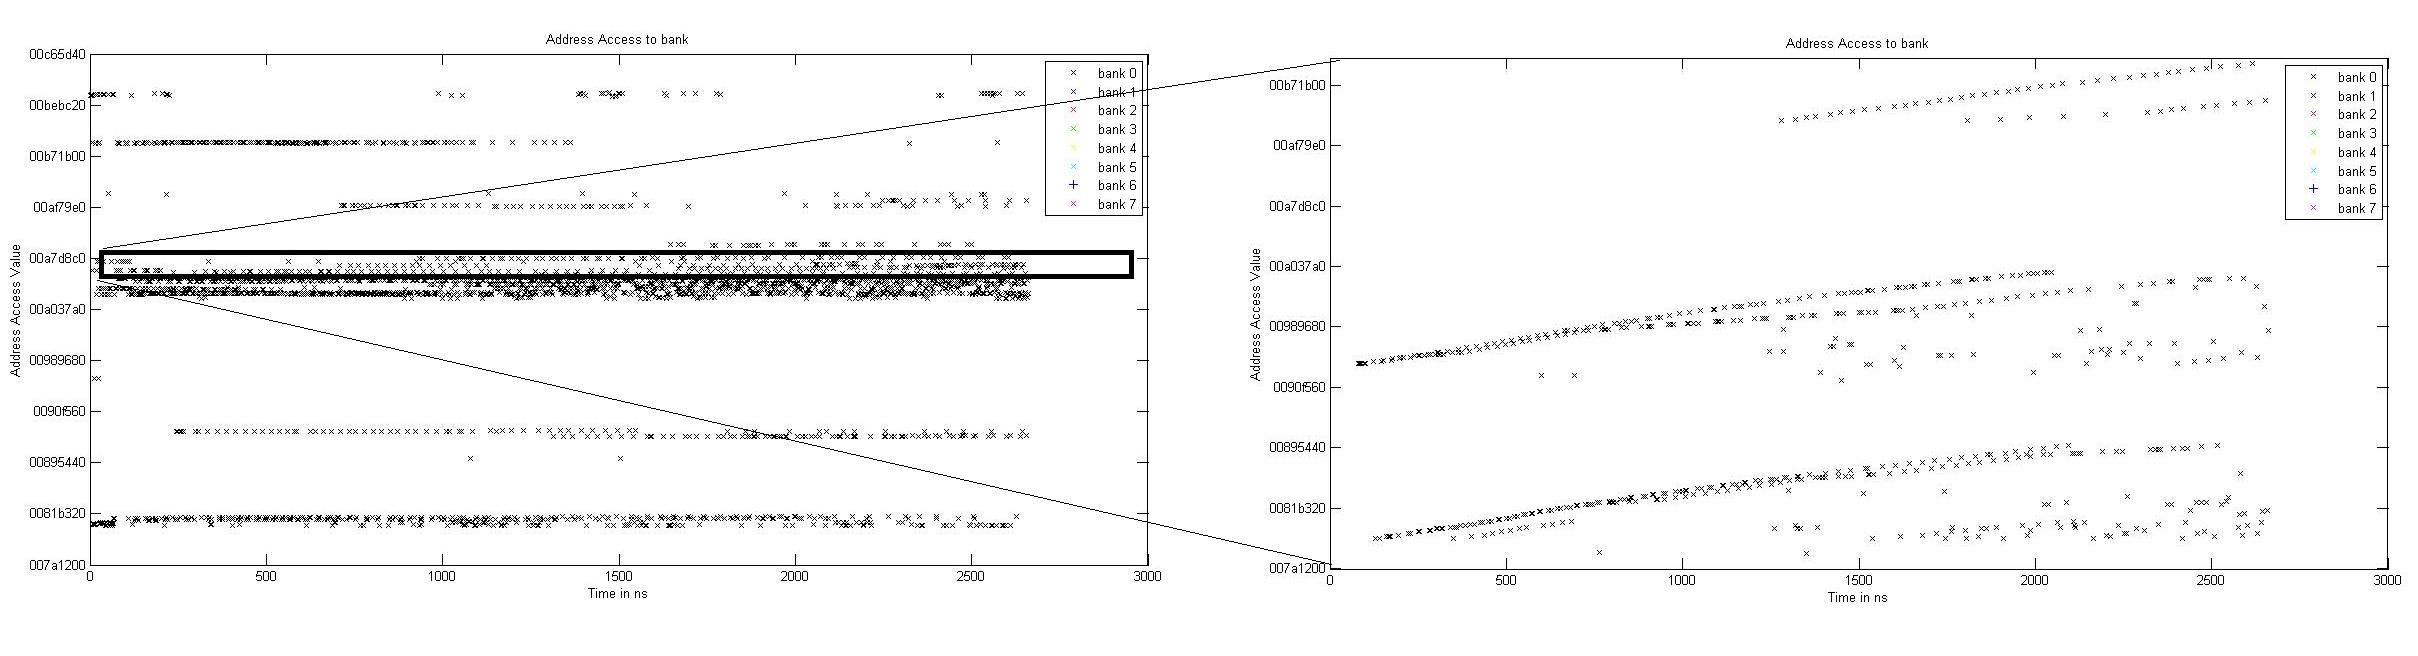
\includegraphics[width=0.5\linewidth]{fig/bank_access1.jpg}
\caption{ }
\label{fig:bank_access1}
\end{figure} Implementation of a memory prefetch should only require overhead 
for space and the associated logic to implement it. Since memory accesses are 
often stalled due to bank conflicts, checking pending accesses to the 
prefetched data should require no additional time overhead. As memory accesses 
wait to be issued in the bank queues, they can simultaneously be checked with 
the prefetched data. Thus, no extra latency is anticipated by the addition of a 
memory prefetching unit.
Figure~\ref{fig:bank_access1} shows two plots of memory accesses to a bank with 
respect to time. The left figure shows the accesses to the memory bank by 
various cores. The right side figure shows a zoomed view of the accesses in the 
dense access region. This figure suggests the linearity of accesses. The system 
can look ahead in the queue to detect the consecutive address request for a 
memory bank and schedule a prefetch of the associated code.  In 
figure~\ref{fig:queue_lookahead}, we simulate the prefetching of the code by 
using a window of length ??. That is, we look ahead to ?? requests in the queue 
and find out the occurrence of consecutive address in the window. The plot 
suggest high occurrence of the consecutive addresses in the bank which can be 
served by prefetching the codes.  
%-----------------------------------
\begin{figure}[htbp]
\centering
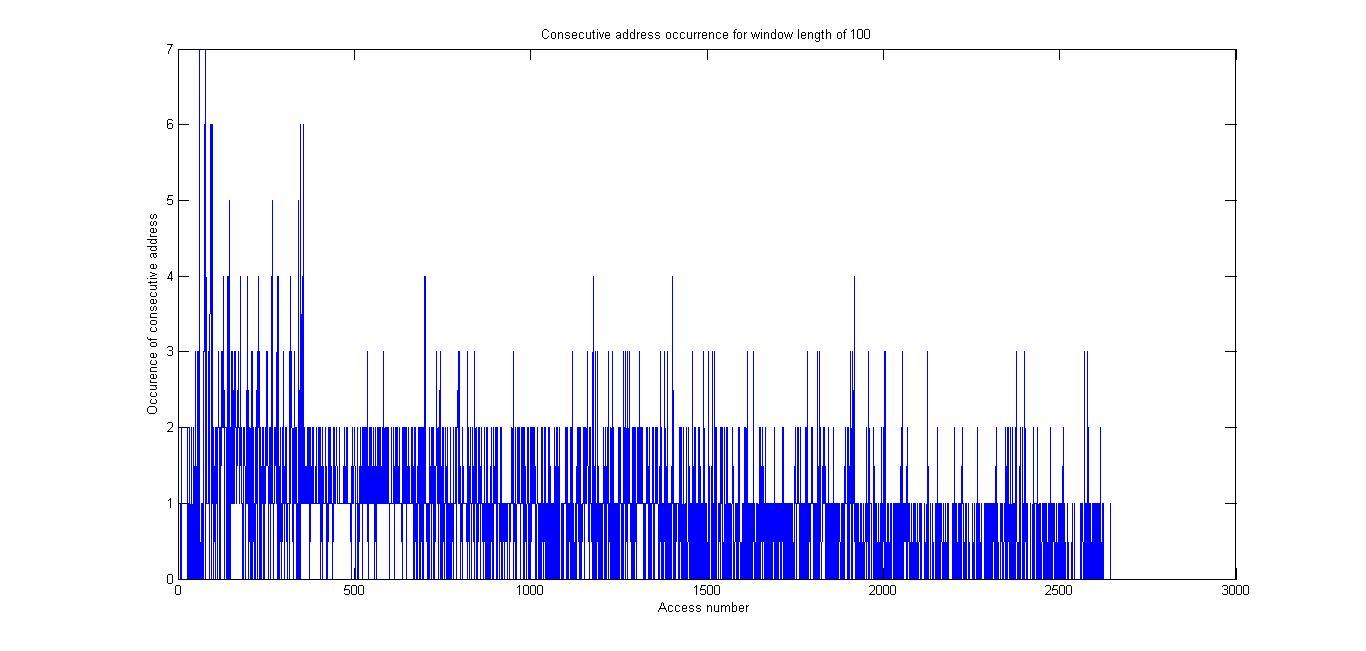
\includegraphics[width=\linewidth]{fig/queue_lookahead.jpg}
\caption{ }
\label{fig:queue_lookahead}
\end{figure} 
%-----------------------------------
%}
%\ignore{
 
%}
